% The document class marks this as a thesis, supplying various options that

\documentclass[ % the name of the author
                    author={Sam Phippen},
                % the name of the supervisor (preferably including title)
                supervisor={Dr. Rafal Bogacz},
                % the thesis    title (which cannot be blank)
                     title={Real time voice activity detectors in noisy personal computing environments},
                % the thesis subtitle (which can    be blank)
                  subtitle={},
                % the degree programme (from BSc, MEng, MSci, MSc and PhD)
                    degree={MEng},
                % the year of submission
                      year={2012} ]{thesis}

\usepackage{parskip}
\usepackage{textcomp}
\usepackage{csvsimple}
\usepackage{rotating}
\usepackage{float}
\floatstyle{boxed}
\restylefloat{figure}
\widowpenalties 1 10000
\raggedbottom


\begin{document}


% =============================================================================

% This section simply introduces the structural guidelines.  It can clearly
% be deleted (or commented out) if you use the file as a template for your
% own thesis: everything following it is in the correct order to use as is.

% =============================================================================

% This macro creates the standard UoB title page, with information drawn
% from the document class (meaning it is vital you select the correct
% degree title and so on).

\maketitle

% After the title page (which is a special case in that it is not numbered)
% comes the front matter or preliminaries; this macro signals the start of
% such content, meaning the pages are numbered with Roman numerals.

\frontmatter

% This macro creates the standard UoB thesis declaration; on the hard-copy,
% this must be signed by the author in the space indicated.

\makedecl

% LaTeX will automatically generate a table of contents, and also associated 
% lists of figures, tables and algorithms.  The former is a compulsory part
% of the thesis, but if you do not require the latter they can be suppressed
% by simply commenting out the associated macro.

\tableofcontents
\listoffigures
\lstlistoflistings

% The following sections are part of the front matter, but are not generated
% automatically by LaTeX; the use of \chapter* means they are not numbered.

% -----------------------------------------------------------------------------

\chapter*{Executive Summary}

\vspace{1cm}

The objective of this project was to build a voice activity detector (VAD)
system, specifically one that was able to differentiate keyboard noise and
mouse clicks from human speech. We targeted this specific problem because
we found that existing VAD systems would transmit keyboard and mouse noise
as voice.

We performed research into why this problem might exist, based on our research
we found that most voice activity detection systems were only attempting to
differentiate voice from background noise. This caused these systems to
transmit anything that was not part of the continuous background noise.
Keyboard impulses definitely fall into this category because they are neither
of stationary amplitude or periodic.

We feel that we have thoroughly solved this problem. We have tested random
forests, gradient boosted regression trees, decision trees and $k$ nearest
neighbor classifiers against each other in a VAD context, determining that
random forests give the best classification results. We have created a database
of some 225000 samples with both voice, keyboard noise and background noise.
The database contains 9 speakers. The resulting classifier that we describe in
this project achieves a 98\% classification accuracy, as measured by the area
under the receiver operating characteristic curve metric.

The main achievements and contributions of this project are:

\begin{itemize}

    \item We built a number of tools in Python for manipulating raw audio.

    \item We designed an accurate VAD system, which is particularly
        effective at dealing with keyboard noise.

    \item We performed research into features that do and do not help
        with our specific VAD problem.

    \item We performed a comparison of classification algorithms with our
        feature set.

    \item We have built a portable VAD corpus that presents a new problem for
        VAD systems.

\end{itemize}


% -----------------------------------------------------------------------------

\chapter*{Supporting Technologies}

We used the following technologies to build our system:

\begin{itemize}

    \item The Python programming language.

    \item The Scikit Learn library: \url{http://scikit-learn.org/stable/}.

    \item The Scikit Talkbox library:
        \url{https://pypi.python.org/pypi/scikits.talkbox}.

    \item The Pylab libraries: numpy, scipy and matplotlib:
        \url{https://www.scipy.org/Getting_Started}.

    \item The Audacity audio editor: \url{http://audacity.sourceforge.net/}.

\end{itemize}

% -----------------------------------------------------------------------------

\chapter*{Notation and Acronyms}

\vspace{1cm}

\noindent

\begin{quote}
\noindent
\begin{tabular}{lcl}
    VAD                 &:     & Voice Activity Detection                 \\
    VOIP                &:     & Voice Over IP\\
    FFT                 &:     & Fast Fourier Transform\\
    PSD                 &:     & Power Spectral Densities\\
    GBRT                &:     & Gradient Boosted Regression Trees \\
    LPC                 &:     & Linear Predctive Coding \\
    ROC                 &:     & Receiver Operating Characteristic \\
    MAE                 &:     & Mean Absolute Error \\
    ZCR                 &:     & Zero Crossing Rate \\
    AUC                 &:     & AUC \\


%DES                 &:     & Data Encryption Standard                \\
%                    &\vdots&                                         \\
%${\mathcal H}( x )$ &:     & the Hamming weight of $x$               \\
%${\mathbb  F}_q$    &:     & a finite field with $q$ elements        \\
%$x_i$               &:     & the $i$-th bit of some bit-sequence $x$ \\
\end{tabular}
\end{quote}

% -----------------------------------------------------------------------------

\chapter*{Acknowledgements}

\vspace{1cm}

This thesis would not have been possible without the continual support of my
supervisor {\bf Dr Rafal Bogacz}, who has spent many hours with me this year giving
me advice on how to organise the execution of this project, as well as ideas
for how to make improvements when I was stuck.

I would also like to thank:
\begin{itemize}

    \item My friend and mentor {\bf Dr Ben Fields}, who spent a couple of his
        afternoons discussing my thesis with me, and also for sharing his
        personal experience of writing 3 theses of his own.


    \item My friend {\bf Alistair Lynn}, who helped me proofread the majority of this
        document.

    \item My good friends {\bf James Laverack} and {\bf Luke Murray} with whom
        I spent a huge amount of time unwinding when I felt burnt out.

    \item My {\bf parents}, who provided me with a much needed supply of tea
        during the long writeup of this thesis.

\end{itemize}

% =============================================================================

% After the front matter comes a number of chapters; under each chapter,
% sections, subsections and even subsubsections are permissible.  The
% pages in this part are numbered with Arabic numerals.  Note that:
%
% - A reference point can be marked using \label{XXX}, and then later
%   referred to via \ref{XXX}; for example Chapter\ref{chap:context}.
% - The chapters are presented here in one file; this can become hard
%   to manage.  An alternative is to save the content in seprate files
%   the use \input{XXX} to import it, which acts like the #include
%   directive in C.

\mainmatter

% -----------------------------------------------------------------------------

\chapter{Contextual Background}
\label{chap:context}

\vspace{1cm}

The term voice activity detection (VAD) \footnote{Sometimes referred to as voice
endpoint location\cite{Tuske}} refers to the algorithms that are used to
distinguish frames of audio that contain speech from those that contain
background noise\cite{ramirez}. The motivation for this project is that we
found, based on personal experience, that existing VAD algorithms struggle to
efficiently distinguish the noise commonly associated with personal computers,
such as typing and mouse clicks, from speech.

\section{Applications}

The two main applications of VAD systems are Voice over Internet Protocol
(VOIP) and Speech Recognition. These systems have to deal with microphone input
and have a strong need to determine whether or not human speech is present in
any particular frame of audio. These systems are not concerned with all of the
audio within the sequence. As such it seems intuitive to build a detector that
can remove frames of audio that do not contain speech.

\subsection{Speech Recognition}

Speech recognition systems are responsible for working out what is being said
in a given sequence of audio. They must be robust to different speakers,
environments, hesitation, stuttering and other human factors. It is often noted
that these systems degrade rapidly in the presence of noise\cite{Moreno}.
Increasingly with systems like Siri\texttrademark\cite{siri} (Apple's speech
recognition system for iOS\texttrademark) people are using systems that require
accurate detection of what is being said. This mostly happens in potentially
noisy outdoor environments.

Speech recognition systems can have their accuracy improved\cite{shin} by
employing VAD systems, which are used to locate speech endpoints. The speech
endpoints are then passed into the speech recognition system. This means that
the system only has to search the places that the VAD system has marked as
containing speech, rather than the entire sequence of audio. If the VAD system
is sufficiently sensitive it may also be able to accurately locate the pauses
between words the user makes. This enables the speech recognition system to
assume 1 or very few words will lie within each part of detected speech, this
helps to improve speech detection accuracy.

A motivating example for improving speech detection accuracy by using an
improved VAD algorithm can be found in \cite{ramirez-2}. They built a
specialised detector that improved over the G.729 ITU-T\cite{itut} standard.
They tested against the well known Aurora\cite{aurora} speech recognition
benchmark suite, using the same speech detector with the two different VAD
algorithms. They found that, with an improved VAD algorithm, they could improve
the number of words correctly recognized by 17\% in the best case.

In the context of this project we believe that our detector may be able to
improve speech recognition through improved voice activity detection. This is
very much a secondary goal. We believe that, in a personal computing
environment, it is more likely that a user is going to be using VOIP than
speech detection.

\subsection{VOIP and Telephony}

When used in a VOIP context VAD systems are used to prevent the transmission of
noise within a conversation. This is typically achieved by setting the
amplitude of any frames that are detected as noise to zero. Often VAD is a
component in a VOIP system that also includes: noise filtering and compression.
The Mumble\cite{mumble} system, for example, includes both an amplitude and a
signal-noise ratio based VAD. The output of the VAD is then passed into the
CELT\cite{celt} codec. In Mumble the VAD system silences any frames detected as
noise and CELT efficiently compresses the silence to ensure a bandwidth saving.

VAD algorithms allow for large bandwidth savings during both analogue
telephone calls and VOIP calls. The reason for this bandwidth saving is that in
both dialogue (two people speaking) and monologue (one person speaking) much of
the time of the call is occupied by silence. Specifically: 60\% of the time is
occupied by neither person speaking\cite{shah} in a dialogue and 20\% of the
time is occupied by neither person speaking in a monologue.

In the case of a traditional analogue telephone call: bandwidth is measured by
counting the total number of slots on wires that are being taken up by a number
of calls. The bandwidth saving is achieved by "Time Assigned Speech
Interpolation" whereby a link can carry more calls by assigning resources only
to those calls that currently have someone speaking on them. This will cause a
significant saving. For example: if speech is only travelling in one direction
only 1 slot can be allocated instead of 2. Another way a saving is achieved is
by allocating no slots to the call when neither party is
speaking\cite{5016247}.

With a VOIP call, a significant bandwidth saving is achieved by nature of the
fact that if transmission were continuous, both parties would be transmitting
at least 64,000 bits per second\cite{ciscovad}. If we assume that for most of
the call only one person is speaking, and that our VAD is sufficiently good at
distinguishing noise from human speech then we will find at least a 50\%
bandwidth saving. Additionally if there are pauses in speech a VAD will
provide an even greater bandwidth saving.


\section{Problem Definition}

Seeing that both user experience can be improved, and that bandwidth savings
can be achieved through the use of voice activity detection systems, the
question is what can be done to improve these VAD systems. The specific goal of
this project is to build a voice activity detection system which is robust in
the typical environment of a modern computer user. Typically these environments
do have a low level of background noise. However, these environments do,
typically, suffer from the problem of irregular high amplitude noise impulses
that are caused by the user typing on a keyboard or clicking a mouse.

We believe that the problem in modern systems exist because most VAD algorithms
are designed for noisy background environments\cite{shin}, but they are not
designed for short, loud noise impulses. These noise impulses are common when a
user is typing on their keyboard. There are two modern consumer VOIP systems
that we used, both were found to transmit keyboard noise and mouse noise  as if
they were someone speaking. The systems were: Mumble\cite{mumble}, a low
latency system designed for gamers to communicate whilst playing with each
other, and Skype\texttrademark\cite{skype}, a well known consumer VOIP solution
designed for single or many person VOIP calls.  Especially in the case of
mumble it is essential that keyboard noise is filtered out, as gamers tend to
be using their keyboards continuously whilst playing video-games. This noise
could possibly drown out much of the real communication or cause annoyance.

The high-level objective of this project is to build a robust voice activity
detector system that can accurately distinguish voice from keyboard and mouse
noise with suitable processing performance for use in real time systems. More
specifically the concrete aims are:

\begin{enumerate}

    \item Survey existing VAD systems for accuracy against our dataset

    \item Build a corpus of Voice/Background Noise/Keyboard Noise that can be
        used to train our VAD system against. We also aim to ensure that this
        corpus can be used by others for future research.

    \item Design a feature representation for our VAD system that is amenable
        to a high classification accuracy.

    \item Work to develop our own algorithm based on machine learning
        techniques and using common features from literature

    \item To, where necessary, optimise the implementation to ensure that it
        can train in an acceptable amount of time, and classify audio in real
        time or faster.

\end{enumerate}



% -----------------------------------------------------------------------------

\chapter{Technical Background}
\label{chap:technical}

\vspace{1cm} 

\noindent

%\section {danpagematter}
%This chapter is intended to describe the technical basis on which execution
%of the project depends.  The goal is to provide a detailed explanation of
%the specific problem at hand, and any previous or related work in the area 
%(e.g., descriptions of supporting technologies, existing algorithms that 
%you use, alternative solutions proposed).  
%
%Put another way, after reading this chapter a non-expert reader should have 
%obtained enough background to understand what {\em you} have done, and then
%assess how novel, challenging and rigorous your work is.  You might view an 
%additional goal as giving the reader confidence that you are able to absorb 
%and understand research-level material.

The basic problem any voice activity detector is trying to solve is the
question of whether or not a particular frame of audio does or does not contain
speech.

In nearly all recording environments there is continuous background noise and,
when there is speech, the microphone picks up speaking on top of that. Thusly
the output of a VAD system is a single bit (1 or 0 for voice or any other noise
detected). In a VAD system we take input from the microphone and then attempt
to determine which of two classes we are in, corresponding to whether we
should or should not transmit the audio further. We formulate this as a
decision as is shown in figure ~\ref{fig:decision1}.

\begin{figure}
        \[ decision = \left\{ \begin{array}{ll}
                    1 & \mbox{if input like $n + v$: speech present}\\
            0 & \mbox{if input like $n$: no speech present}.\end{array} \right. \]


                    Where $n$ represents the presence of background noise and $v$ represents the
                    presence of conversational speech. This is referred to as additive
                    noise\cite{sohn} and generally represents a very realistic model of most
                    environments in which human speech must be differentiated from background noise.

                    \caption{Decision model for most voice activity detectors}
                    \label{fig:decision1}

\end{figure}


In this project our problem definition is slightly different: we do not only
deal with background noise, we also deal with the fact that keyboard noise is
picked up by microphones. This noise is in no way stationary: while most people
do type with some rhythm, it is not entirely periodic. Additionally the noise
can vary with speed of impact and many other factors. Moreover we have
to deal with the case where someone is typing and talking at the same time.
The decision we have tried to model is stated in  figure \ref{eqn:decision 2}.

\begin{figure}
\[ decision = \left\{ \begin{array}{ll}
            1 & \mbox{if input like $n + k + v$: speech present}\\
            0 & \mbox{if input like $n + k$ or $n$: no speech present}\\

    \end{array} \right. \]
            Where $k$ represents the keyboard noise component of the input.
            \caption{Decision model for our voice activity detector}
            \label{eqn:decision 2}
\end{figure}

This problem definition is different to the classical VAD problem for the
reasons specified above. This is due to the highly non-stationary nature of
keyboard noise. It is worth noting that this model is still entirely additive.
This model is used in many of the papers we have referenced. We believe that
this model accurately reflects our problem as the sources of noise should not
destructively interfere with each other. It is, however, worth noting that an
additive model does not take into account the phenomenon of clipping. Clipping
can occur when the input level to the microphone exceeds its limit. In this
case the additive model breaks down, we did not encounter clipping in our
experiments.

Nearly every existing voice activity detector makes the assumption that
background noise is continuous, if irregular in volume and frequency. These
systems attempt to distinguish voice from the background noise. More commonly
than not we have found that these detectors merely identify any sound that is
not part of the continuous background noise, giving real scope to our project.
Specifically identifying sudden impulses of sound from the background, and
determining whether or not they are someone speaking or someone typing is the
main aim of our system.

\section{Understanding voice}

In particular there are two types of speech, voiced and unvoiced speech. The
easiest way to demonstrate the difference between this is to place two fingers
on your throat/lower chin and then make a ``sssssssss'' sound (unvoiced) followed
by a ``zzzzzzzzzzzz'' sound (voiced). In the first example one cannot feel any
vibration, however in the second example one feels ones throat vibrating.
Voiced and unvoiced speech have somewhat different characteristics and this
must be taking account of when building a VAD system\cite{atal}.

The fundamental frequency of human speech is in the 75-150Hz range for men and
the 150-300HZ range for women\cite{Traunmüller}. However, human speech also
contains many harmonics, this means that there are a number of other frequency
peaks in recordings of human speech. The voice band, the band used for
transmission of speech lies in the 300HZ to 3400Hz range. Some think that this
frequency range might cut off the sound of speech, due to starting above the
fundamental. Enough of the harmonics are included in this band that much of the
fidelity is not lost. The listener will get the impression that they are
actually hearing the missing fundamental tone.

To explain the harmonic content of voice is it necessary to understand how
harmonics of a fundamental note work. The harmonics of the fundamental are
integer multiples in frequency of the original note, demonstrated in figure
\ref{img:harmonics}. We see that the first harmonic is the wave with a base
frequency, the second harmonic is with twice that frequency and so on. Due to
the complex physics of how our bodies force air through our throats we get a
large frequency response not only at the fundamental notes of voice, but also
at the first few harmonics of the fundamental.

We can see that a section of voice features strong harmonics of the fundamental
in figure \ref{img:spectrogram} a spectrogram, showing the frequency strength
over time for a segment of speech. Specifically with the first word note the
strong fundamental at 600Hz with strong harmonics at 1800Hz (3rd harmonic) and
2400Hz (4th harmonic).

\begin{figure}
    \center{
    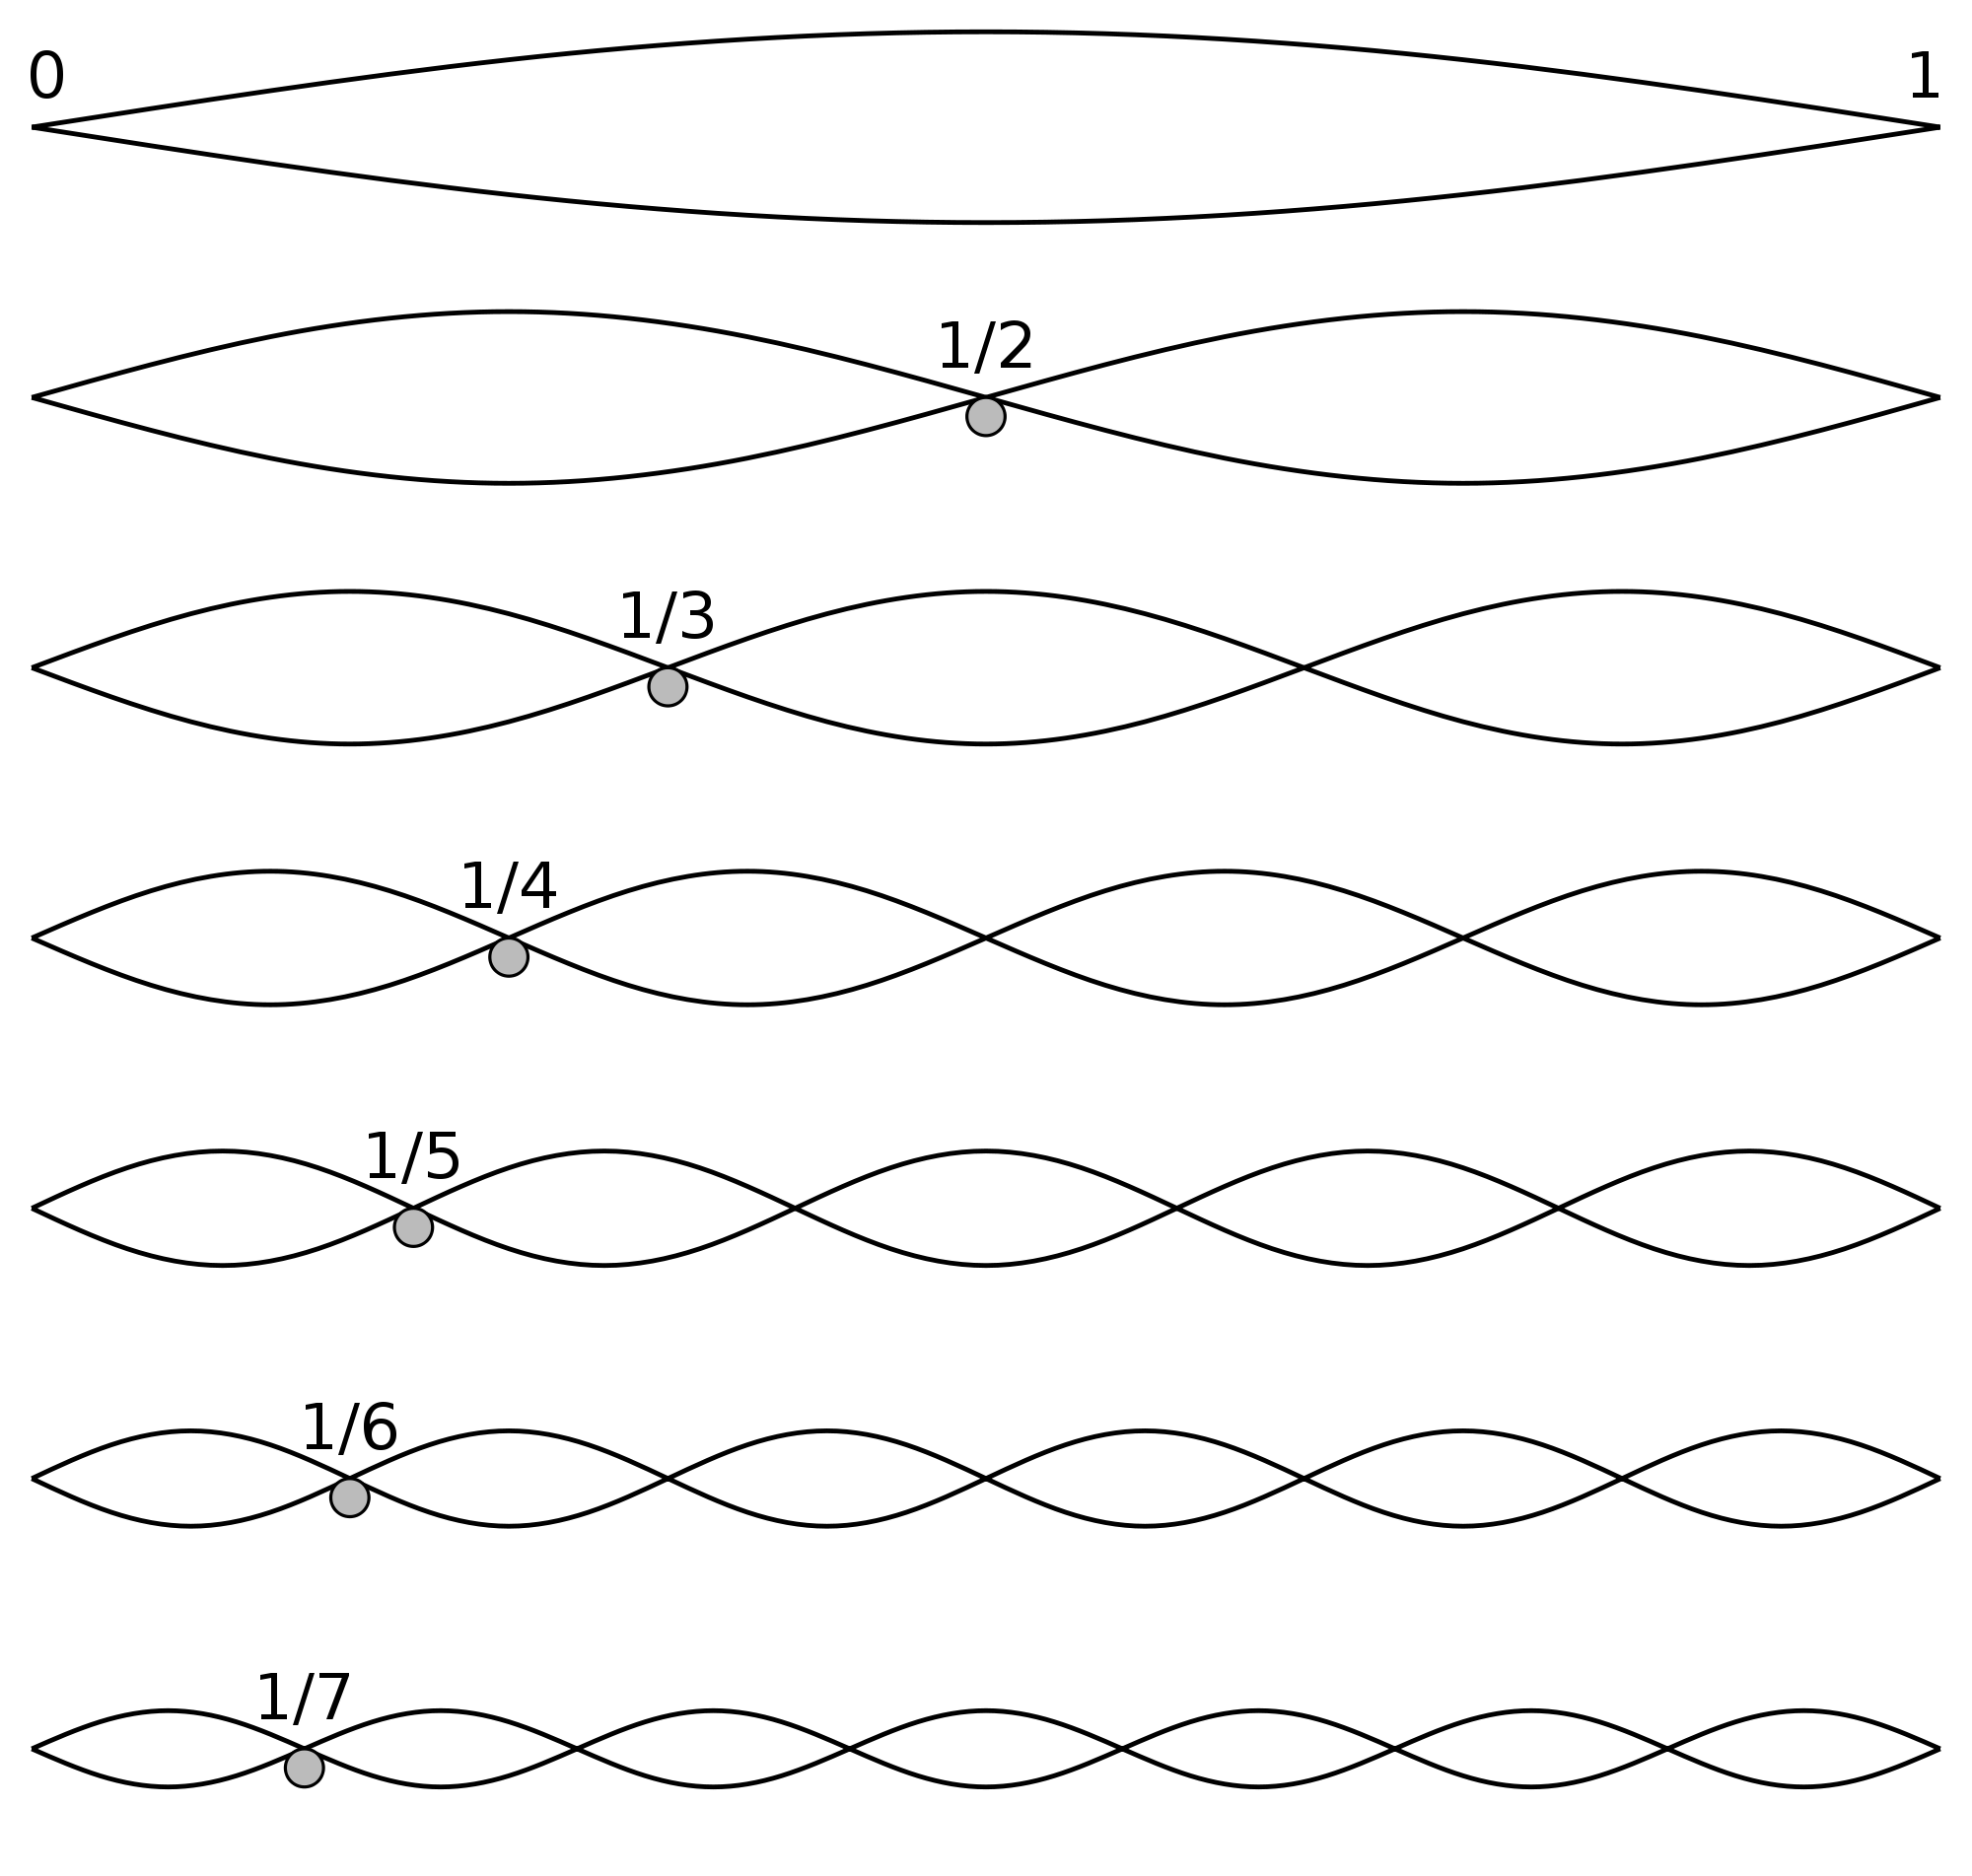
\includegraphics[height=10cm]{harmonics.png}
}
    \caption{A demonstration of the harmonics of a fundamental frequency}
    \label{img:harmonics}
\end{figure}

\begin{figure}
    \center{
    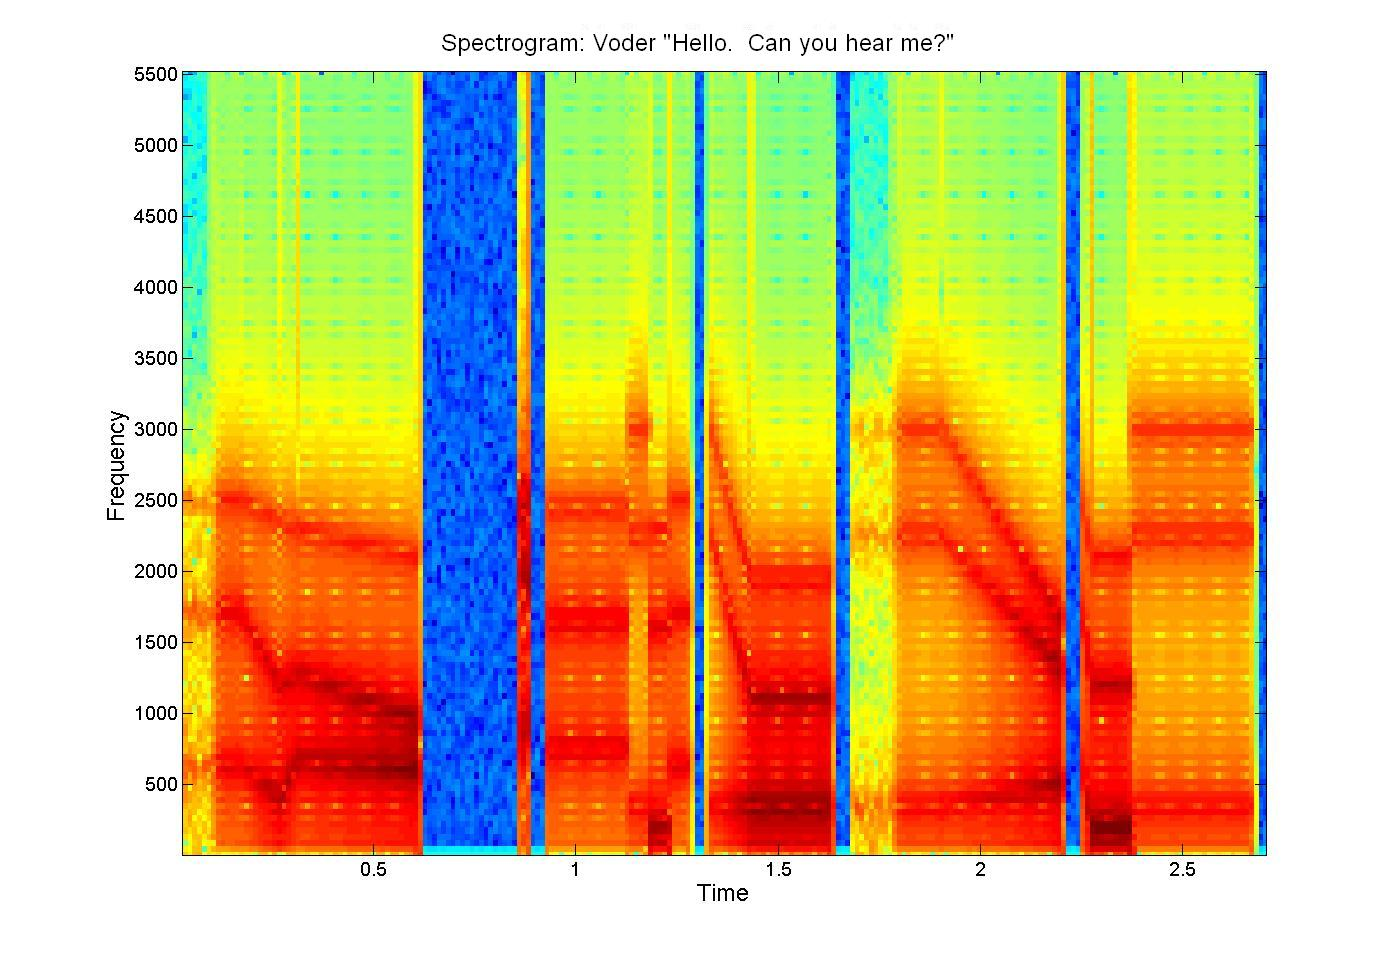
\includegraphics[height=10cm]{voder_spectrogram.jpg}
}
    \caption{Spectrogram of voice harmonics with speech}
    \label{img:spectrogram}
\end{figure}

\section{Existing Voice Activity Detection Techniques}

Existing voice activity detection techniques fall into one of two categories.
The algorithms are either threshold based, or use machine learning techniques.
Threshold based algorithms use a number of parameters from the audio being
transmitted. Each parameter is given a threshold (the noise/voice threshold). A
decision over all the parameters is made, using the thresholds, as to whether
the audio is or is not voice. In some systems the thresholds are static with
the thresholds determined experimentally over some training data\cite{haigh}.
These systems, by their design have trouble dealing with background noise that
changes such as computer fans spinning up/down, or a person using a mobile
phone walking through streets with different environmental noises in the
background.

In other threshold based voice activity detection systems the thresholds are
adaptive\cite{gokhun}. These systems are designed to deal with non-stationary
background noise, that is background noise that changes in amplitude and pitch.
These systems usually start with an initial guess of their class thresholds
which then change over time. The thresholds change based on the running average
of each of the parameter values for the two classes, as output by the
detector\cite{sakhnov}.

The other major class of voice activity detectors apply machine learning
algorithms to build a complex classification boundary over the parameters of
the model\cite{shin}. These classifiers can suffer from the problem of having a
static decision boundary. This static decision boundary is due to the fact that
on-line training is not possible. This is usually not an issue due to the fact
that the more complex decision boundary achieves a much higher accuracy when
trying to decide between the voice and non-voice class.

\subsection {Features}

In both threshold based and machine learning based VAD systems a number of
features are extracted from the raw audio. These features are used to build a
representation of the audio that can be used in the decision systems and is
likely to easily distinguish speech from non-speech. In this section we
investigate existing features that are used in models for voice activity
detection, including those that were and were not used in our model.

\subsubsection{Commonly used features}

In this section we investigate some of the features that are commonly found in
other VAD systems. The motivation for this is to find features that can be used
in our classifier to give a good representation for the classifier to be
trained against. Our problem definition is, admittedly, slightly different to
the common VAD case. Specifically we have extremely non-stationary background
noise. Features from other systems may be useful in building our VAD system.
This section also serves to define how features are constructed for when these
features are referred to later on in this paper.

One of the most commonly used features in voice activity detection is the
energy of a window. The equation for energy is given in figure
\ref{eqn:energy}\footnote{ sometimes also implemented as the root mean square
of a window}, this feature is used in
\cite{shin}\cite{sakhnov}\cite{gokhun}\cite{haigh}\cite{atal} and \cite{sohn2}.
The energy feature of a particular window of audio has been found to be
significantly higher in frames that contain speech than background
noise\cite{atal}. This parameter also forms different distributions for voiced
and unvoiced speech. The energy values for voiced speech are typically
significantly higher than those for unvoiced speech. In \cite{atal} they state
``The energy of unvoiced sounds is usually lower than for voiced sounds, but
often higher than for silence.'' The system they used was a threshold based
system, while in \cite{shin} this feature was used as part of a machine
learning based system.  They reported ``The full band energy, the conventional
feature for endpoint detection for clean speech, does not work well for noisy
speech.'' The feature did, however, give roughly 88\% accuracy figure by itself
when used in their classifier. This feature was used in our system for
classification.

\begin{figure}
    $$Energy(x) = \sum_{i=0}^{length(x)}x_i^2$$
    \caption{Energy of a window x, where length(x) gives the number of individual
    \label{eqn:energy}
    samples in x}
\end{figure}

Another commonly used feature in voice activity detection is the zero crossing
rate of a window. The definition for this feature is given in figure
\ref{eqn:zero-crossing-rate}. This feature is not used in \cite{shin}, but is
used in \cite{atal}. In \cite{atal} it is stated that zero crossing rate varies
consistently with energy. For the classifier based system that we are building,
it is very important to find features that vary from each other. The reason for
this is that if the features have low correlation they are very likely to give
``statistically independent'' views on the data. When this happens the classifier
is able to take advantage of these statistically independent views to give a
significantly higher classification accuracy. In \cite{shin} they state that
zero-crossing does not perform well in noisy speech, they did not use this
parameter at all and did not make any actual reports on the accuracy of the
feature. In \cite{haigh} they found that a detector based on energy and
zero-crossing rate only failed in noisy conditions. This feature was also used
in our detector.

\begin{figure}

    $$ZeroCrossingRate(x) =
    \sum_{i=1}^{length(x)}abs(sgn(x_{i-1})-sgn(x_i))$$


    Where x is the signal, sgn gives the sign (-1, 0 or 1) of a value and
    abs gives the absolute value of a value.

    \caption{Zero crossing rate of a frame}
    \label{eqn:zero-crossing-rate}
\end{figure}

\subsubsection{Other features from existing systems}

There are a number of other features that were used in the system we built that
came from existing implementations of voice activity detection. We here explain
these features so that the reader is aware of how the feature values are
calculated.

Another feature that is used in \cite{shin} is referred to as a ``band energy''.
This simply takes the energy as specified in figure \ref{eqn:energy} but
instead of computing it over the entire window, it is taken over the amplitude
component of a Fourier transform that has had a band pass applied to it, with
the frequency band specified.  An example of this is the
300-3700Hz band energy\footnote{This range corresponds to the audible range of the
telephone system} that Shin et al refer to. This band energy is
computed by taking the sum of squared amplitude values of the components of a
Fourier transform that lie within the 300-3700Hz frequency range. In our system
we used multiple band energies which are discussed in chapter
\ref{chap:execution}.

In \cite{haigh} they used cepstral features for voice activity detection. There
are multiple transforms that are referred to as the ``cepstrum'' of a signal,
specifically the complex cepstrum, the power cepstrum and the phase
cepstrum\cite{childers}. The power cepstrum is defined in figure
\ref{eqn:power-cepstrum}. This feature is primarily used in speech recognition,
the higher order task of determining what words are being said, rather than
voice detection\cite{muda}. In \cite{atal} they criticize this approach for
VAD, stating that this feature requires a very high degree of periodicity
(signal approximately repeats itself with a fixed period) to provide an
accurate classification.

\begin{figure}
    $$PowerCepstrum(f)=|\mathcal{F}^{-1}\{\mbox{log}(|\mathcal{F}\{ f_t \}|^2)\}|^2$$
    \caption{Definition of a power cepstrum. $f$ is our
    signal function, $\mathcal{F}$ is the Fourier transform function. $|a|$}
    \label{eqn:power-cepstrum}

\end{figure}

Specifically in \cite{haigh} they use a cepstral distance measure,
\footnote{Euclidian distance} between testing samples and a training set of
samples. The classification was given as the class of the sample in the
training set which was nearest to the sample being classified. This is
equivalent to a single nearest neighbor classifier. They did not report an
accuracy figure, however they did include a diagram which shows that their
classifier was configured to be particularly sensitive. This probably means
that they were able to get an accurate classification in stationary background
noise. This approach would probably not work for our problem class.

In \cite{moattar} one of the key features that they extracted was the dominant
frequency component of the signal. This corresponds to the highest peak in the
Fourier transform of the signal and is defined in figure \ref{eqn:dom-freq}.
The authors of the paper observed that this feature was helpful in
discriminating speech and silence frames. We observed problems with this
feature due to the nature of our windowing system which are discussed in
chapter \ref{chap:execution}. The accuracy of this feature is reported in
\cite{moattar} to have a greater than 80\% accuracy under even noisy
conditions. The main caveat that they point out with this feature, that the
background noise must be in someway regular, does not apply to our project. Our
noise is highly irregular and is almost certainly not of stationary amplitude.

\begin{figure}
    $$DominantComponent(f) = argmax_i(|\mathcal{F}(f_t)|)$$

    $f$ is the signal
    function, $\mathcal{F}$ is the Fourier transform. $argmax$ gives us the
    input corresponding to the maximum output of a function.
    \caption{Definition of the dominant component of a signal}
    \label{eqn:dom-freq}
\end{figure}

In \cite{atal} they used two features constructed via a linear predictive
coding (LPC) analysis. The basic principle of linear predictive coding is that
the current sample can be approximated as a linear combination of the previous
samples\cite{rabiner}. One representation of the LPC is the coefficients
($a_1,a_2,...,a_p$) that are used to generate the prediction. In \cite{atal}
they specifically used a size 12 linear combination, which means that each
sample was predicted as a linear combination of the previous twelve. It is
important to note here that over short periods of 10-30ms voice signals are
roughly periodic, and that it is obvious that $s(n) \approx s(n-N_p)$ where
$N_p$ is the length of the period. LPC techniques work with window sizes that
are significantly smaller than the period and still accurately reconstruct the
next part of the signal. The result of the LPC is a number of coefficients that
can be used to attempt to reconstruct parts of the signal. These coefficients can
also be used as parameters to both threshold and classifier based systems. In
\cite{atal} they used two parameters from the LPC:

\begin{itemize}

    \item The first coefficient of a 12 coefficient LPC analysis: this is the
        primary coefficient $a_1$ of the LPC analysis, corresponding to the
        sample nearest to the sample we are trying to predict.

    \item The energy of the error in the prediction made by the LPC. This is
        essentially defined as the error signal (computed by subtracting the
        signal predicted by the LPC and the actual signal). Energy is defined
        above as the sum of the squares of the signal in figure
        \ref{eqn:energy}. In the paper they state that this feature is
        equivalent to the ratio of the geometric mean of the spectrum to the
        arithmetic mean of the spectrum. This makes it equivalent to the
        spectral flatness measure defined in \cite{moattar}.

\end{itemize}

\subsection{Power Spectral Density}

The power spectral density of a signal is a transform that is similar to the
fourier transform. The power spectral densities give the relative power per
frequency, for several frequency components of the signal. The power spectrum
does, however, differ from the fourier transform in a couple of key ways.
Firstly the power spectrum has no phase component, it only gives the absolute
power/frequency values for each component. Secondly the fourier transform gives
us the relative strengths of sinusoids in a signal. The power spectrum is
effectively a fourier transform of the autocorrelation function, this means
that it gives us the relative strengths of long and short term correlation
within the signal .\cite{psd}\cite{psd2}


\section{Machine learning techniques}

In this project we decided to use machine learning techniques to build our VAD
system. This is primarily due to the fact that threshold based approaches
report lower accuracy rates in the literature and are very much designed to
differentiate continuous background noise from sudden changes in any of their
parameters. Our feeling was that this would not be amenable to differentiating
sudden keyboard impulses from sudden voice impulses. In the execution chapter
of this project we discuss how we built the classifier and training set for
this system, and this section specifically conducts a review of machine
learning systems, with an explanation of state of the art machine learning
techniques such as random forests, gradient boosted regression trees and
adaboost with decision stumps. All classifiers here are discussed under the
assumption that they only have to deal with a binary classification problem,
which corresponds to the classification problem that we are dealing with
(voice/non-voice classification).

\begin{figure}
    $$\text{Train}:(R^x \times R^y) \times \{0,1\}^y \rightarrow \text{ModelFunction}$$

    y is the number of classes. The function takes an x by y matrix of reals
    and a y-length vector of labels and outputs a model function that behaves
    as a classification function defined in in figure \ref{eqn:define-classify}

    \caption{Definition of a training function} x is the number of features and

    \label{eqn:define-train}
\end{figure}

\begin{figure}
    $$\text{Classify}: R^x \rightarrow \{0,1\}$$

    x is the number of features, the model takes a feature vector and outputs a
    class, in some implementations this may be a probability instead of a {0, 1}
    classification.

    \caption{Definition of a trained model/classification function}

    \label{eqn:define-classify}
\end{figure}

\subsection{Classification and regression trees}

Classification and regression trees are class of machine learning algorithm
that train a binary decision tree over the training samples. They classify by
pushing examples through the binary decision tree. Training is performed by
computing splits in the feature space. Typically, these splits are chosen to
give the best possible improvement in classification rate, assuming that the
training set is totally representative. At the start the split that gives
highest information gain over the entire data set is chosen, giving us two
subsets of the entire data set, these subsets are then split recursively as if
they represented a new entire training set. This process continues until the
leaf nodes of the tree give a classification of homogeneous class. By this
method we ensure that all training examples will be classified correctly, in
general this method can lead to some over-fitting that will cause the classifier
to not generalise as well, and the trees are pruned. An example decision tree
is shown in figure \ref{fig:decision-tree}.

\begin{figure}

    \center{
        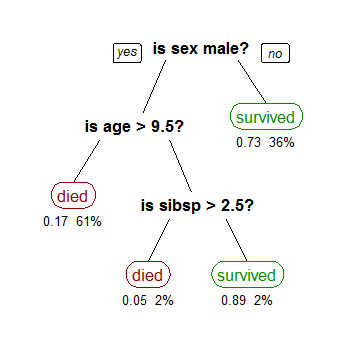
\includegraphics[height=10cm]{decision_tree.png}
    }

    \caption{An example decision tree kindly provided by Wikipedia}
    \label{fig:decision-tree}
\end{figure}

Regression trees are used when the output is not a single class but instead
some single real number. For example a regression tree might be used in an
attempt to predict the length of a patient's stay in hospital. In \cite{shin}
individual features were passed through a speech/non-speech classification, and
then a CART (classification and regression tree) was employed over the outputs
of the pre-classifiers to come to the final decision. This approach gave a very
high accuracy level under low and medium noise levels (-5dB and 0dB
respectively) but degraded under high noise levels (5dB). In this system they
further improved their classification accuracy by passing in: the current window
to be classified, the previous window that had already been classified and the
next window to be classified.

\subsection{Decision Stump}

Whilst never used on its own the decision stump classifier is worth exploring
due to its use in ensemble\footnote{Ensemble classification methods are a class
    of classification algorithm that combine many classifiers in an attempt to
    improve classification accuracy or generalizability or both. In chapter
\ref{chap:evaluation} we show that these methods give much better accuracy than
non-ensemble techniques with some intuition for why this is the case.}
classification methods. Specifically the decision stump classifier acts like a
normal binary decision tree classifier or CART. Instead of training recursively
with many splits, it is trained for only one split. These often achieve very
low classification accuracy and are sometimes referred to as ``weak'' or ``base''
classifiers. In the famous Viola Jones face detector\cite{viola} many decision
stumps were used to form a strong classifier that achieves very good
classification accuracy. An example decision stump is shown in figure
\ref{fig:decision-stump}.

\begin{figure}

    \center{
    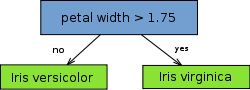
\includegraphics[width=5cm]{decision_stump.png}
}


    \caption{An example decision stump kindly provided by Wikipedia}
    \label{fig:decision-stump}
\end{figure}

\subsection{Adaboost}

Adaboost is a well known\cite{viola}\cite{sun2006reducing} 
algorithm for ensemble classification that achieves a
high classification accuracy by training many base classifiers. Unlike some of
the other ensemble methods that we discuss in this paper the Adaboost method
can be used with any base classifier. Due to this it may be useful in a larger
set of problems than other ensemble methods presented here. Specifically, the
result of training an Adaboost classifier is a chain of classifiers. The later
classifiers in the chain tend to be more biased towards the most difficult
samples to classify within the training set.

The final classification output of the Adaboost algorithm is given as a linear
combination of weights multiplied by the classification output\footnote{The
    classification output of the classifiers within the Adaboost chain is
usually either an integer class or a real posterior probability} of each of
the individual classifiers within the Adaboost classifier. The pseudocode
for training the system is given in figure \ref{pseudo:adaboost}.

Within this project we use an Adaboost algorithm that uses decision stumps as
its base classifier, this decision was made based on the fact that we wanted
training to complete quickly (decision stumps train in effectively no time) and
that this approach has been shown to work well in other problem
domains\cite{viola}.

It is worth noting that training an Adaboost classifier with a very large
number of weak classifiers can cause a high level of overfitting, especially
in the presence of noise within the data set\cite{sun2006reducing}.

\begin{figure}
    Pseudocode for training an Adaboost classification system. It is important
    to note that the weak classifiers must be sensitive to the weights given in
    the $w$ array. If the classification system that is used is not sensitive
    to these weights (for example a decision tree by default has no concept of
    weighting its inputs) we can weight the samples by performing a roulette
    wheel selection\footnotemark on the samples.

    \vspace{3em}

    \begin{enumerate}

        \item let $w_1(i)=\frac{1}{N_{samples}}$ for all $i$ in
            $0,1,...,N_{samples}$.

        \item for i = 0 to number of classifiers in ensemble (n)
            \begin{enumerate}

                \item Train a weak classifier that returns -1 or 1 given a
                    sample.
                \item Choose $\alpha_i \in R$.
                \item Update $w(i) = w(i)exp(-\alpha y_i h_t(x_i))$ for all $i$ in
            $0,1,...,N_{samples}$.
            \item Normalize $w(i)$ so that it sums to 1 (forms a probability distribution).

            \end{enumerate}
        \item output strong classifier: $$H(x) = sgn\left(\sum_{i=0}^{n}\alpha_i h_i(x)\right)$$
    \end{enumerate}

    \vspace{3em}

    In step 2a in the previous listing we specifically pick the weak classifier
    that gives the lowest weighted prediction error over all the samples, where
    the weighted prediction error is defined as: $$error_{h_i} =
    \sum_{k=0}^{N_{samples}} w(k)(y_k\neq h_i(x_k))$$By doing this at each
    stage we are effectively picking the weak classifier that is most capable
    of dealing with the most highly weighted samples. This gives us an improved
    classification over a single classifier because the difficult samples are
    given "specialist" classifiers that are more capable of dealing with them
    than a classifier trained over the entire set.

    In step 2b we specifically chose $\alpha_i$ to greedily minimize
    classification error at each step, that is at every step the overall
    classification error on the training set will go down rather than up.

    \caption{Adaboost training psuedocode and explanation}
    \label{pseudo:adaboost}

\end{figure}
\footnotetext{Roulette wheel selection is an algorithm which
        allows us to select randomly from a weighted array. If the array forms
        a probability distribution (that is that it sums to 1) then we can
        generate a number uniformly at random and move through the array of
        weights, subtracting each weight from the generated number, when the
        number reaches zero we have arrived at the item that corresponds to the
    randomly generated number, and we can output it. When performing this
selection multiple times we end up with a distribution of selections from the
array that matches the weights of the items.}

\subsection{Random Forest}
\label{section:random-forest}

The random forest classification algorithm is a modern ensemble method for
classification proposed by Breiman in \cite{breiman}. In a random forest many
decision trees are combined, this give a much better classification result than
any single decision tree is able to. In order to arrive at a final class the
original Breiman paper suggested that the classifier's output should be the
modal class of the classifiers in the ensemble.  In this project the
implementation of our random forest classifier is slightly different. Each tree
in the ensemble computes a posterior probability. Instead of giving a modal
class output, the mean of posteriors is taken to give a more sensitive
classification. The output is thresholded to 0.5000 for the voice/non-voice
classification. This implementation may give a more accurate classification due
to the fact that it can take into account the relative confidences of each of
the decision trees.

The training method for a randomised forest as described in \cite{breiman} is
to create a randomised vector from the training set by performing selection
without replacement at random from the training set. This means that any single
instance may occur more than once in the randomised vector. This is the same
technique that is used in the bagging ensemble classification method. In our
system the randomisation is taken a step further, we also train each tree in
the ensemble on a, different, randomised subset of the features of the training
set.

There is a second class of random forest used in this paper called extremely
randomised trees. This method goes one step further in the randomisation during
training. The extremely randomised forest algorithm does not split on the most
discriminative threshold of the most discriminative feature of a random subset
of the features. Instead, the extremely randomised forest picks $n$ random
thresholds of each feature in the random subset of features and then picks the
one with the highest information gain.

In figure \ref{fig:comparison} we can see a comparison of decision trees,
random forests, extremely randomised trees and Adaboost. It is worth noting
that the decision boundaries for random forests are a lot noisier around noisy
data than the other classification algorithms.

\begin{figure}
    \begin{center}
        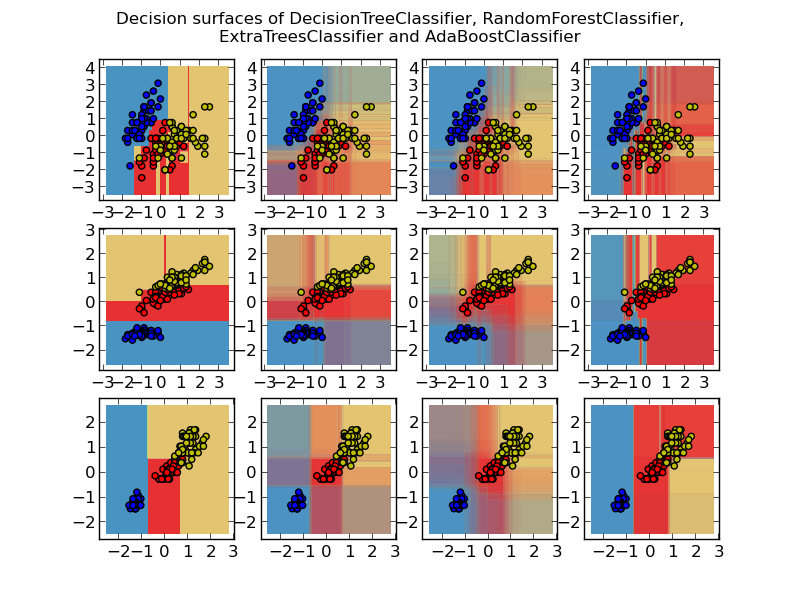
\includegraphics[width=13cm]{classifier_comparison.png}
    \end{center}

    \caption{Comparison
    of decision trees and ensemble classification techniques}

    This shows data points with circles and decision boundaries with background
    colour; shading in the background colour indicates probability where the
    ensemble methods have internal classifiers that disagree. The decision tree
    always has block color as it gives a single class as an output rather than
    a probability. Specifically this plot shows the various classifiers being
    trained against a single dataset with different features. The columns
    are the decision surfaces for the various classifiers. The rows are the
    different representations of the dataset, with differing features.

    \label{fig:comparison}

\end{figure}

\subsection{Gradient Boosted Regression Trees}

The gradient boosted regression trees (GBRT) algorithm uses boosting to build a
strong classifier, it trains many decision trees over the training set.  The
output of the GBRT (Gradient Boosted Regression Trees) is computed in a similar
fashion to Adaboost. They both take the sum of the outputs of the classifiers
in the ensemble, multiplied by some weight associated with each classifier. 

The difference between this technique and Adaboost is in how we change the
treatment of samples in each iteration. In Adaboost more difficult samples are
given a higher weight. In GBRT we change the class label on each sample to be
the residual between the original class label and what the current ensemble
classifier outputs for that sample.

The main disadvantage of GBRT in comparison to the Random Forest technique is
that the training process cannot be easily parallelized. This is due to the
fact that each new tree must be trained as a function of the ensemble
classifier that has been trained thus far.

In \cite{parker} they use GBRT to perform sequence alignment of music, this
technique was also used by the winning submission to the Netflix prize.

\subsection{A review of ensemble techniques}

The ensemble techniques that we have discussed so far all have been shown to
perform significantly better in generic machine learning applications than
single classifiers. This is because they build a number of different models,
with either a randomised component, or a dependency on moving against the error
of the ensemble. These techniques however come with a high processing
performance overhead. This is simply due to the fact that there are many
classifiers instead of one. Adaboost with decision stumps does somewhat serve
as an exception to this rule because decision stumps take virtually no time to
perform a classification. In this thesis we consider decision trees, random
forests, gradient boosted regression trees and Adaboost, comparing the feature
set that we developed in an attempt to maximise accuracy and generalizability.
Classification performance  served as a secondary concern because many of the
performance problems in our system were not in the classification layer.

\section{ROC Curves}

A ROC curve, or Receiver Operating Characteristic curve, is a curve that is
used for evaluating the accuracy of a classifier by comparing the false
positive and true positive rate. The area under the ROC curve can also be used
as a measure of the accuracy of the classifier. In a 2 class problem a
completely random classifier will strike a line between (0,0) and (1,1). Better
classifiers tend to move towards better true positive rates and lower false
positive rates and typically occupy the upper left half of the ROC curve. An
example of this can be seen in figure \ref{fig:roc-example}. Note how several
thresholds are pointed out on the curve.

The reason for these thresholds is that most classifiers do not output a binary
class decision. They give a posterior probability or some other likelihood that
the example belongs to a specific class. By thresholding the decision boundary,
we can affect both the true positive and false positive rate. This is
particularly important in classifiers that aren't merely going for raw maximum
classification accuracy, but rather care about a decision one way or the other.
For example in our classification problem it would be disastrous if some voice
were not transmitted when the user was speaking, so our system will naturally
fall to the lax threshold rather than the strict threshold.

\begin{figure}
    \begin{center}
        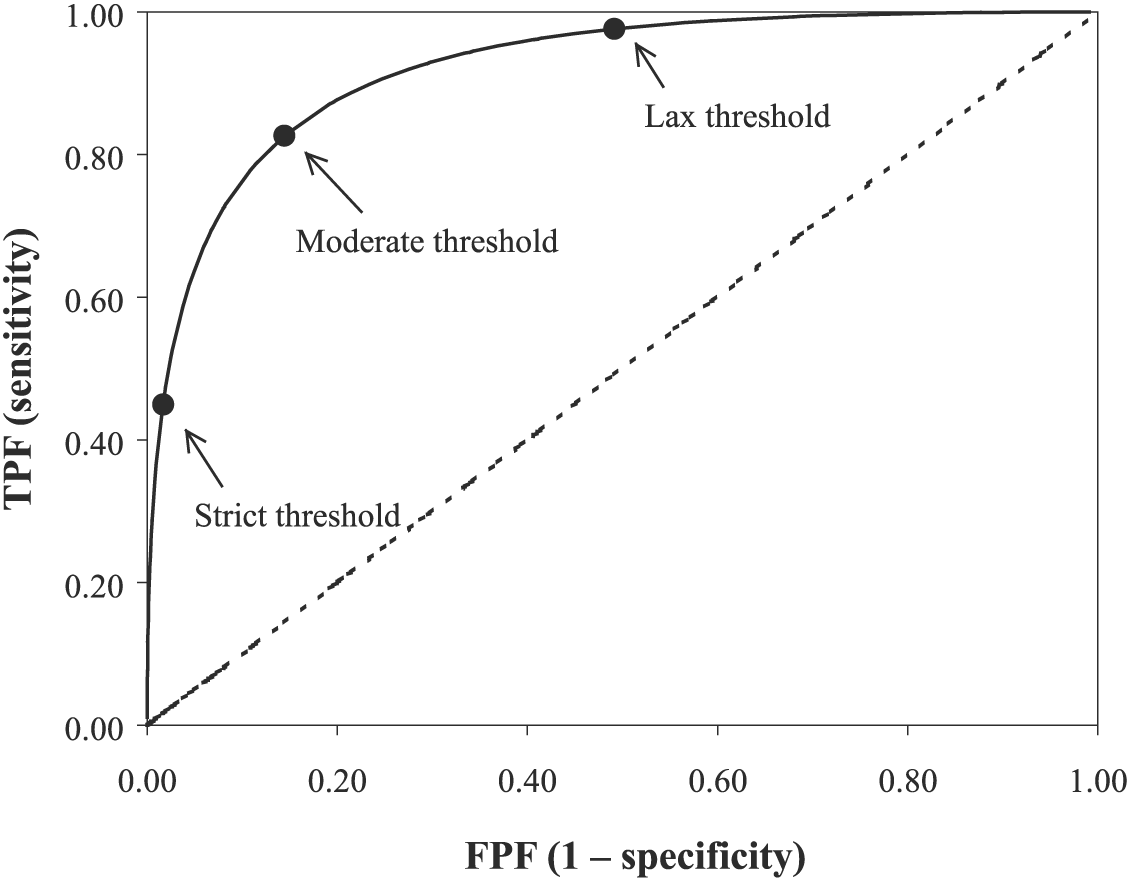
\includegraphics[height=10cm]{roc_example.png}
    \end{center}
    
    Axes are False Positive Frequency $(x)$ and True Positive Frequency $(y)$.
    
    \caption{An example ROC curve}
    \label{fig:roc-example}
\end{figure}

The area under the ROC curve is a measure of the predictive power of the
classifier\cite{fawcett}. No classifier used in the real world will have an
area under the ROC curve of less than 0.5000, as random guessing will always
produce a diagonal line between (0,0) and (1,1). The specific meaning of the
AUC (area under the curve) statistic is: the area under the curve is the
probability that the classifier will rank a randomly chosen positive example
more highly than a randomly chosen negative example.

\section{Mean absolute error}

Later in this paper we refer to the mean absolute error, MAE, of a classifier.
The mean absolute error is computed by taking the mean of the absolute
differences between the predicted and actual class labels, for each instance
that the classifier is being tested against. An equation for this is given in
figure \ref{mae-eqn}

\begin{figure}
    \begin{center}
        $$MAE(predictions, actual) = \sum_{i=0}^n\frac{abs(predictions(i)-actual(i)}{n}$$
    \end{center}

    Where predictions and actual are two arrays of binary labels of length n.
    \caption{Equation for mean absolute error}
    \label{mae-eqn}
\end{figure}



% -----------------------------------------------------------------------------

\chapter{Project Execution}
\label{chap:execution}

\vspace{1cm} 

%\noindent
%This chapter is intended to describe what you did: the goal is to explain
%the main activity or activities, of any type, which constituted your work 
%during the project.  The content is highly topic-specific, but for many 
%projects it will make sense to split the chapter into two sections: one 
%will discuss the design of something (e.g., some hardware or an algorithm), 
%inc. any rationale or decisions made, and the other will discuss how this 
%design was realised via some form of implementation.  
%
%This is, of course, far from ideal for {\em many} project topics.  Some
%situations which clearly require a different approach include:
%
%\begin{itemize}
%\item In a project where asymptotic analysis of some algorithm is the goal,
%      there is no real ``design and implementation'' in a traditional sense
%      even though the activity of analysis is clearly within the remit of
%      this chapter.
%\item In a project where analysis of some results is as major, or a more
%      major goal than the implementation that produced them, it might be
%      sensible to merge this chapter with the next one: the main activity 
%      is such that discussion of the results cannot be viewed separately.
%\end{itemize}
%
%\noindent
%Note that evidence of ``best practice'' project management (e.g., use of 
%version control, choice of programming language and  so on) should only 
%be included if there is a clear reason to do so.

\section{Building the dataset}

One of the most important problems that we had to solve, in order to build our
classification based VAD system, was to build a dataset that is representative
of our problem. We also have to ensure that the dataset can easily be ingested
for use in a classifier. In this section we will discuss our approach to
constructing a dataset that allows us to achieve the aims outlined in this
thesis.

The first step in building the dataset was to record a reasonable amount of
audio that can be used to build the classifier. In order to build our sample
database we used the recording feature of the Mumble\cite{mumble} program. We
connected to the Mumble server for the Computer Gaming Society of the University of
Bristol Students union. Due to the fact that there were multiple players during
each session, we were able to capture separate recording channels for each
player in the game. In total this database amounts to 24 hours of audio,
although not all of this audio was used in the overall classification system.
The audio captured was of extremely high quality at 48kHz with 24 bit samples.
This was compressed down to 16 bit samples at 48kHz for use in this project due
to the large memory requirements of loading the entire set.

It is worth noting at this point that while there are existing datasets such as
the Buckeye corpus\cite{buckeye}, none of them contain noise that comes from
keyboard and mouse inputs. This being the critical target of our project. It is
also worth noting that due to the large number of people that were involved
with the recording we get a large number of different microphone/keyboard/mouse
configurations. This is useful to build a classifier that is robust to these
different configurations. Additionally it is worth noting that there is a minor
gender imbalance in this dataset, with 10 males and only 1 female in the
dataset. Whilst this may cause the classifier to generalise less well, the
dataset was recorded from the best available source at the time.

Once the audio had been recorded the task of labelling presented itself.
Initially this labelling was performed by opening the audio in the audio editor
Audacity\cite{audacity} and then selecting regions of audio and playing them
back. This approach had the advantage of allowing relatively large, continuous
regions to be labelled quickly. The disadvantage was that it was a very slow
process when there were short regions where people would utter short words and
then return to the silence/typing class.

In order to speed this process up a simple Python script was written with a
very simple class detector. The script makes a best guess by running over
200ms windows of audio, detecting whether the sum of the absolute value of each
of the frames in the window was above some very low threshold. If the sum of
the current window was the same side of the threshold as the previous window,
then they were joined together. This meant that the smallest audio window that
the user had to label was 200ms. The longest windows occurred when there was
contiguous speech, which based on labelling experience were around 4 seconds.
An example waveform with a contiguous region of 2.6000 seconds, followed by a
200ms region, the shortest region of homogeneous class, is given in figure
\ref{img:labelling_example}.

This script allowed for background noise to be separated from both sharp
keyboard impulses and people speaking. The user was then interactively asked to
label the audio by hand. In addition to the interactive labelling windows of
total silence were simply given a homogeneous background noise
label\footnote{due to the fact that frames with 0 amplitude clearly do not
represent someone speaking}. The labelled data was stored in an sqlite
database, represented by: the start time, end time, original file name and the
class label. The advantage of this approach is that it allowed for quick
labelling of a lot of data for our classifier. This approach did, however, have
the disadvantage that some 200ms regions contained audio of multiple classes.
We feel that this problem did not affect the training set too much, due to the
very high classification accuracy that we achieved.

Another advantage to this approach is that we have stored the audio and the
class label information separately. This meant that we were able to apply
transformations to the raw audio data, without affecting the accuracy of the
labelling. This was useful when we started performing experiments such as
changes in bits per sample and frame rate\footnote{These changes have some
important affect on classification accuracy}. It is also worth noting that we
did not end up labelling all 24 hours of audio that was available. This would
taken an incomprehensibly large amount of time. Additionally we felt that we
could still build a valid proof of concept classification system with the data
that we labelled. Specifically we have just over an hour of labelled audio,
split amongst all but one of our speakers (one of the males). The distribution
of labelled data amongst the various participants can be seen in figure
\ref{img:speaker_distribution}. The dominant speaker, speaker 7, is the
recording speaker, this speaker was present in every recording session. Speaker
3 is the female speaker and forms a relatively large part of the data set.

\begin{figure}
    \center{
        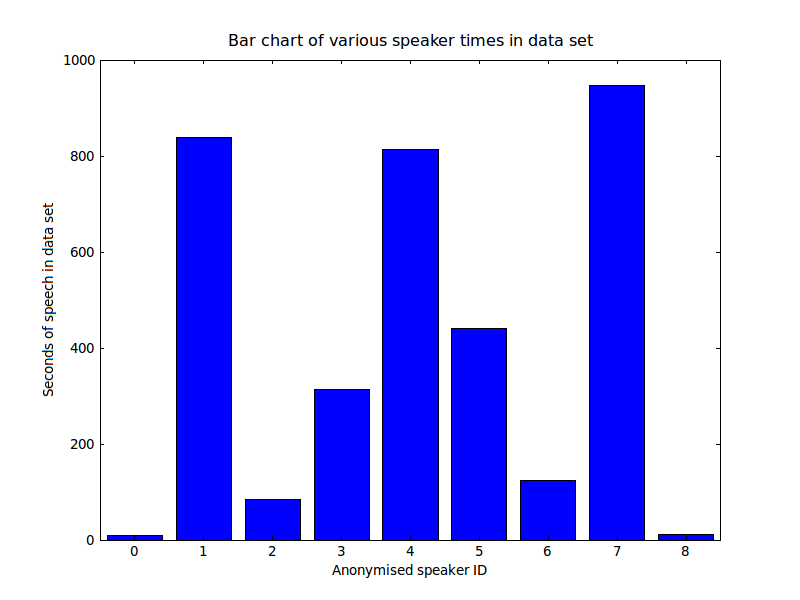
\includegraphics[height=10cm]{speaker.png}
    }
    \caption{Distribution of speakers in the labelled dataset}
    \label{img:speaker_distribution}
\end{figure}

\begin{figure}
    \begin{center}
        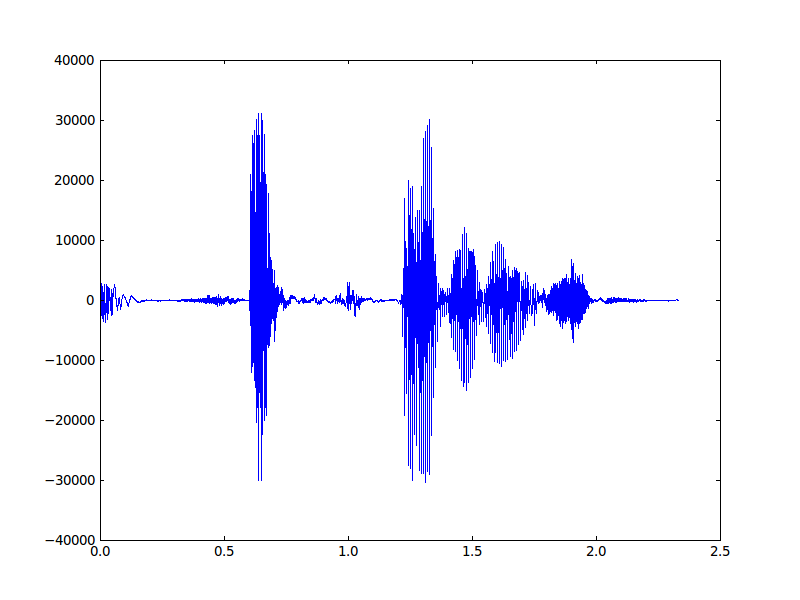
\includegraphics[width=8cm]{labelling1.png}
        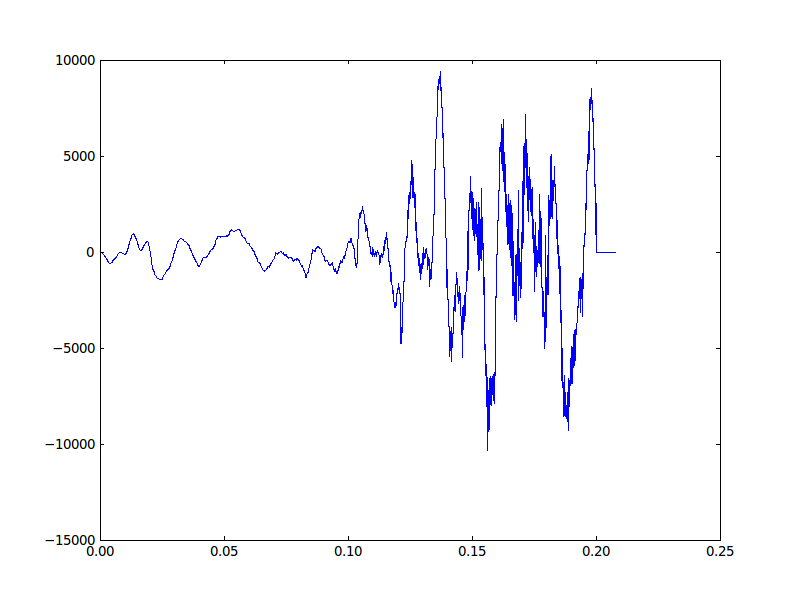
\includegraphics[width=8cm]{labelling2.png}
    \end{center}

    The x axis here represents time in seconds, the y axis here represents the
    amplitude of the sample at that point in time.

    \caption{Example of contiguous and short region in simple labelling system}
    \label{img:labelling_example}
\end{figure}

\section{Building the classifier}

From the start we used the Random Forest classifier discussed in section
\ref{section:random-forest}, this is due to both familiarity and availability.
Specifically we took an off the shelf implementation from the
scikit-learn\cite{sklearn} Python library. This library was chosen due to its
general popularity and the author's familiarity with Python. Once the
classifier had been chosen we decided to classify on windows of 16ms. This
window length was chosen because it is used in gaming applications as the
target frame rate for any on screen graphics. This frame rate corresponds to 60
frames per second, which most players perceive to be acting in real time. The
background research indicates that this frame size is not outside the desired
range of 10-30ms, it is worth however noting that the Shin\cite{shin} system
uses a slightly shorter, 10ms window size.

In this section, classification accuracies are reported as the result of a 10
fold, randomised, stratified cross validation\footnote{There was a minor
    imbalance in the number of samples in each of the classes, with roughly
    53\% background noise and 47\% voice}.  The folds were trained with 66\% of
    the data in the training set, we felt that this split gives a reasonable
    tradeoff between giving the classifier sufficient data to train on, and not
    training in such a way that the classifier would be overly biased towards
    the dataset. In other words we are trying to retain some of the
    generalizability of our classifier by using a 66\% training set rather than
    a 90\% training set\footnote{The 90\% split is standard for a 10 fold cross
validation}.

The general binary classification problem that we formulated in the technical
background chapter of this paper requires that we have some fixed size vector
of real numbers for each sample in the training/test sets. Obviously this means
that we cannot pass some arbitrary length audio stream into the classifier and
attempt to get a result. The first order solution to this problem is to apply a
window the audio. Specifically: we must pick a fixed window size that is short
enough that it will not be perceived as lagging whilst classification is
occurring, short enough that we can classify it in real time \footnote{if our
window contains 1 million samples it is unlikely that we can classify it in
real time}, and long enough that it contains enough information so that it can
be classified.

We initially chose a 16ms window size as the size of the window for
classification, this falls within the common window sizes in the background
literature, which typically fall in the 10ms-30ms. Our specific choice of 16ms
was made because this is the traditional framerate that many gaming
applications target, representing 60 frames a second. This is traditionally
perceived as smooth by most gamers. Our initial choice of 16ms, with the 48kHz
audio that we use gives us 768 samples per window. Initially we decided to pass
all 768 samples as a vector as the representation of the window for
classification.

The classifier with 768 samples gave a relatively unsatisfying classification
accuracy of around 77\%, in cross validation. It was obvious that merely taking
the windows and passing them into the classifier would not give an accurate
classification result. The reason for this is that two windows that essentially
represent the same sound could be offset by one sample, the classifier would
treat these as two wildly different samples, despite them having similar
frequency components and other features. We felt that much could be done to
improve the classification accuracy of the system by building a good feature
representation. In order to allow easy construction of a representation of the
audio that would allow for a high classification accuracy, we added another
stage to the pipeline that sat between the audio on the hard drive and the
classifier. Specifically the pipeline had these stages:

\begin{itemize}

    \item For reach row of the database, extract class label, start time, end
        time and file name.

    \item For each of those, open the file for reading and read samples out of
        the file between the start time and the end time.

    \item Cut the sample into 16ms windows, appending 0s if necessary.

    \item Apply all feature transforms to get a uniform width vector of real
        numbers.

    \item Send feature vectors along with class labels into the classifier for
        training.

\end{itemize}

This allowed us to mix feature transformations as the project went on, removing
and adding as necessary. The features that were initially implemented were
based on the research and also some visualization/analysis of the dataset. The
initial feature set we went with was:

\begin{enumerate}
    \item Energy: the sum of squares of the window, referred to in the technical
        background chapter.

    \item Zero crossing rate: the number of times the samples in the window
        change in sign, referred to in the technical background chapter.

    \item The energy of the 3500 to 4300Hz frequency band: implemented as a
        squared sum of the Fourier magnitude domain of the values in this
        frequency band. This feature was implemented due to it corresponding to
        a peak in the average Fourier transform of one of the classes.

    \item The energy of the 5400 to 6800Hz frequency band: implemented as
        above. This feature was implemented due to it corresponding to a peak
        in the average Fourier transform of one of the classes.

    \item The energy of the 1800 to 2700Hz frequency band: this corresponds to
        the most dominant frequencies of voice according to the research.

    \item The dominant frequency in the 300 to 5000Hz band: this is a wide band
        around the fundamental frequency of human voice, up to a very high
        harmonic. Used to attempt to differentiate keyboard noise from voice.

    \item The energy in the 0-100Hz energy band: this band was chosen due to
        the effects of windowing on the Fourier-amplitude domain and is
        discussed further in this section.

    \item The kurtosis of the Fourier-amplitude domain: this is effectively a
        measure of ``peakyness'' of the spectrum.

    \item The energy of the error of an LPC analysis: as discussed in the
        technical background chapter, the LPC has been shown to be a good
        predictor of voice signals. This metric is computed as the squared
        error between the prediction of the LPC and the window.

    \item The 12 coefficients of a $p=12$ LPC analysis: These coefficients
        are essentially a different representation of the result of the LPC
        when compared with the residual mentioned above. Our fear with this
        feature was that they may have a high level of correlation. We have
        extensively compared the correlations of our features below.

    \item The third component of the power spectral density of the signal: this
        component corresponds to a large peak in the average power spectrum.
        This can be seen in figure \ref{fig:psd}.

    \item The dominant component of the power spectral densities of the signal
        above the third component: this feature was determined experimentally
        to be a reasonable weak estimator that separates our negative and
        positive classes.

    \item The sum of the power spectral densities between the $30^{th}$ and $37^{th}$
        components: this feature was determined experimentally to help
        classification as much as any of the other features.

    \item The energy at another peak ($21^{st}$ component) within the PSD of the
        signal: this was also determined experimentally to provide reasonable
        classification accuracy on our problem set.

\end{enumerate}

\begin{figure}
    \begin{center}
        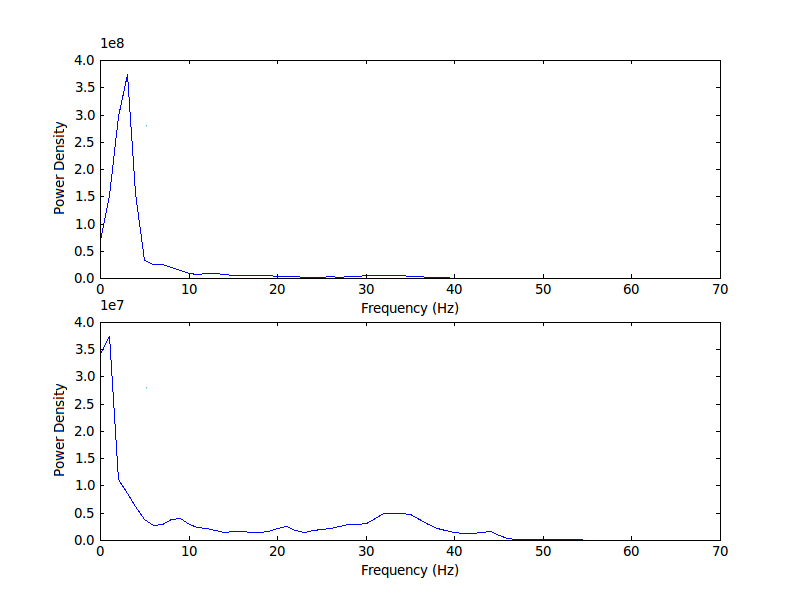
\includegraphics[width=10cm]{psd_plot_last_figure.png}
    \end{center}

    \caption{PSD of voice and noise classes}

    The top plot is the voice class, the bottom plot is the noise class. Note
    that the y axis on the top plot is times ten to the eight and the y axis on
    the bottom plot is times ten to the seven.


    \label{fig:psd}

\end{figure}

Features 2, 3, 4 and 7 are shown along with the complete Fourier amplitude
domain in figure \ref{fig:frequencies}.

\begin{figure}
    \begin{center}
        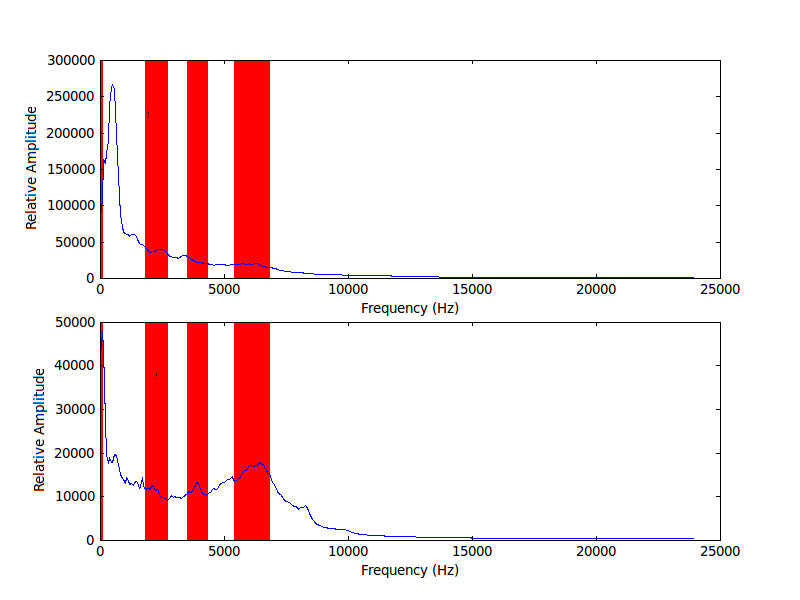
\includegraphics[height=10cm]{frequencies.png} 
    \end{center}

    These plots both show the average Fourier transform for all the audio in
    the two classes.  The voice FFT is the top subplot, and the noise FFT is
    the bottom subplot, with the frequency bands mentioned in 2,3,4 and 7
    highlighted.

    \caption{Histogram of fourier domain for voice and noise classes}
    \label{fig:frequencies}
\end{figure}

As we can see these four frequency bands vary from each other between the two
classes. Specifically we can see that these frequency bands represent spikes in
the noise class and are more flat in the voice class. Additionally we can see
that the relative amplitude at these points is much lower for the noise class
than the voice class. In figure \ref{table:importances}, in the next chapter,
we show the relative feature importances as computed by the classifier over our
original feature set. These give relatively high importances (specifically just
over 11\% of the classification accuracy come from the 3 higher frequency
bands).

Part of the implementation process that was very useful was checking both the
feature correlation and the relative classifier importances of our features.
The reason for this was that it allowed us to reject features that high
correlations or low importances. We have documented these below with reasons
for their rejection.

\begin{itemize}

    \item The mean value of frames in the window. This was found to have very
        poor predictive importance, even with low feature counts. With low
        feature counts this especially bad as predictive importance is
        normalized to sum to 1 regardless of the feature count. Specifically
        the predictive importance was: 0.1\%, some 10 times smaller than even
        our worst predictive importances.

    \item The spectral flatness measure of the power spectrum: in the technical
        background section we indicated that the LPC residual is equivalent to
        the spectral flatness measure of the absolute values of the fourier
        transform. Whilst the power spectrum does differ from the frequency
        spectrum it is somewhat correlated, and as such the SFM of the power
        spectrum was highly correlated ($r=0.841$) with the LPC residual energy.

    \item The energy of the 2-4kHz band. Whilst this feature was used in
        \cite{shin} we found that this feature did not give good predictive
        power. This feature was actually implemented before the energy bands
        that we used in the final classifier. We found that the bands that we
        decided on gave better predictive power for our problem set. We believe
        this is due to both voice harmonics and keyboard noise occupying this
        frequency band.

    \item The dominant frequency of the entire spectrum. This feature was
        originally implemented in an attempt to increase classification
        accuracy. However based on the spectra in figure \ref{fig:frequencies}
        the problem with this feature becomes obvious. Due to the windowing
        process much of the low frequency information gets disproportionately
        represented. This means that this feature would always stop above the
        200Hz value. The features we ended up using specifically take into
        account this spike and attempt to give a much better representation of
        the dominant frequencies in the signal.

    \item After the features that have been described above were implemented in
        the system we investigated adding cepstral features into the system. We
        found that the features from the cepstrum were already accounted for in
        the rest of our features. We also found that they were correlating
        highly with many of the other features in the classifier without
        providing particularly high feature importances. As such they were
        rejected.

    \end{itemize}

It is worth noting that some of the features that we built did not come
directly form the background research given in the technical background section
of this document. Instead they were based on tweaks from the features listed.
For example the FFT Kurtosis metric that we used was inspired by the
"peakyness" feature in \cite{shin}. In \cite{shin} the process for calculating
this feature was not clearly documented. We found two metrics that could be
used to compute the relative peakyness of a distribution. The first is the
spectral flatness measure (flatness being the opposite of peakyness). This
feature was computed on both the Fourier spectrum and the power spectrum. We
rejected it because of its very low classification accuracy. We ended up using
the kurtosis metric because it measures peakedness relative to a normal
distribution, for unimodal distributions\cite{DeCarlo}. Our distributions are
definitely unimodal, they have a peak at the far low components of the spectrum
(see figure \ref{fig:frequencies}).


\section{Classifier Performance}

One of the most important things in our implementation is to ensure that the
performance of the classifier is good enough for application in a voice activity
detection system. Additionally the amount of time taken to train the classifier
is important. Certainly the actual problem that this classifier is trying to
solve is the question as to whether it should, or should not, further transmit
audio to the rest of a VOIP or speech recognition system. This decision must be
made in faster than real time to ensure that there is no perceived lag by the
user.

A certain amount of online training is possible by asking users to use the less
advanced "push to talk" detection system. By using this system the users are
effectively training the system. They effectively indicate which pieces of
audio they do/do not wish to transmit. We believe that our system could be
extended to new users using the push to talk technique for real time labelling.
In the Critical Evaluation section our robustness to unseen speakers is shown
to be less than perfect, so some online training is very much desired.

It is important to consider the processor performance of the classifier, if it
is found to be to slow in either training or classification then some
improvements must be made. There is also a performance concern with our
implementation, specifically we used the Python\cite{python} programming
language which is interpreted and not known for high execution speed. In
addition to this concern we are using the numpy and scipy libraries which are
not compatible with the most stable JIT implementation of Python,
PyPy\cite{pypy}. The JIT implementation, obviously, runs somewhat faster than
the implementation with no JIT.

In this section we document some of the places where optimisations had to be
made. We made these optimisations as otherwise the system would not have a
realistic application in the VAD space. Some of the optimisations are only
useful for use during training over a large database. These optimisations act
on batches of instances (either arrays of samples or Fourier transform
results). Other optimisations are useful both during training and on-line
classification. This is due to the fact that audio coming out of the audio
hardware is buffered, and we can take advantage of there being multiple 16ms
windows of audio in the buffer.

\subsection{Bytes Per Frame}

One of the initial bottlenecks in the implementation of our system was reading
all the audio off the disk into a representation that could be used for
processing. We also faced a bottleneck with applying processing to that
in-memory data. Obviously reducing the size of the audio is a simple way to fix
this problem. We decided that dropping from 24 bit to 16 bit frames was a good
way to fix this problem. Firstly this massively reduced the time to read the
files off the disk (surprisingly by about a third!). It also meant that the
process of reading the audio into an array of numbers was faster. The reason
for this is that routines for reading 16 bit integers from a packed binary
format exist within the Python language, but routines for doing the same to 24
bit integers do not. This meant that we had to read them in as 32 bit integers
and then decode them back into their 24 bit format. This lead to much
additional processing which in a native programming language may not have been
a problem. Whilst this is an obvious drawback of using a high level language
like Python the speed of development far outweighs the performance cost.

One of the first advantages that reducing the bit rate gave was: computing the
Fourier transform and power spectral densities of the audio happened much more
quickly. When working with a non-trivial amount of data (approximately an hour)
this makes an appreciable time saving. Specifically we found that the time
saving was approximately 50\%, when compared with originally processing these
features. We assume this is because we were able to pack the integers into 16
bits and numpy uses SSE vector operations.

Another advantage that this gave was that the classifier was able to train more
quickly. The reason for this is obvious when looking at the specifics of how
our classifier implementation works: it splits all feature domains until they
are fully split. If we reduce the resolution of every feature domain by
reducing the resolution of the input audio we would naturally expect the
classifier to train more quickly.

\subsection{Zero Crossing Rate}

When initially building the first implementation of the system, the performance
bottleneck was not in the training of the classifier. Rather the bottleneck was
the application of the feature transformations to the input audio. One of the
transforms that was taking by far the longest to execute was the zero crossing
rate feature transformation. The reason for this was that in Python iterating
through each element of the audio arrays took an appreciable amount of time.

The Python as it stood then is given in figure \ref{list:zcr-slow}.


\begin{lstlisting}[frame=single,caption=Original slow zero crossing rate implementation, label=list:zcr-slow]  % Start your code-block
    def zero_crossings(self, frame, fft):
        sum = 0
        for i in xrange(1,len(frame)):
            sign1 = -1 if values[i-1] < 0 else 1
            sign2 = -1 if values[i] < 0 else 1
            if sign1 != sign2:
                sum += 1
\end{lstlisting}

This was optimised using the numpy library which is written in pure C, with
optimised SSE instructions, using this library gave a significant speedup. On
the order of taking 4 hours to read the data set was reduced to only 10
minutes. For training numpy also allows one to apply transformations in a
batch. This optimisation was not used for the ZCR feature. However it was used
to perform the Fourier transform over the entire training set. This batch
optimisation will not be used during real time classification: we can only
apply transforms to frames as they come from the input device. For interest the
numpy python code for the zero crossing rate feature is given in
figure \ref{list:zcr-fast}.

\begin{lstlisting}[frame=single,caption=Numpy fast zero crossing rate implementation, label=list:zcr-fast]
    def zero_crossings(self, frame, fft):
        return len(numpy.where(numpy.diff(numpy.sign(frame)))[0])
\end{lstlisting}

\subsection{Windowing process}

The windowing process that broke the continuous streams of audio into 16ms
windows was, initially, also written in pure python and was very slow. This is
a problem that affects both the real world and training/test scenarios that we
have. This is because the audio from the hardware data stream is not provided
as single frames but is rather buffered to achieve better throughput. We should
expect between 2048 and 16384 frames of audio at a time\footnote{corresponding
    to 40ms to 340ms of lag, depending on the quality of the audio
hardware that is being used}. Being able to perform a batch transformation of
the audio to 16ms windows very quickly is very important.

The initial pure Python implementation of windowing was sufficiently fast with
a small training set. It took only a few minutes to execute, however this
performance degraded very much linearly with the amount of audio that had to be
processed. When the data set grew to around an hour this was far too slow. The
original Python code is given in figure \ref{list:windowing-slow}. Note that in
this implementation the audio is padded with zeros until it meets a round
number of window lengths. This choice could have potentially degraded accuracy,
but seemed better than trying to read the rest of the audio from the file. If
the samples did not come to a round number of windows, the next part of audio
had been labelled with a different class. Also given that we trained with 200ms
wide windows this means that only $1$ in every $12$ windows would suffer from
this problem.


\begin{lstlisting}[frame=single,caption=Original slow windowing implementation, label=list:windowing-slow]
def samples_to_16ms_frames(samples, framerate=48000):
    build = []
    ptr = 0
    frames = []

    while ptr < len(samples):
        ptr += 1
        if ptr % frame_size == 0:
            frames.append(build)
            build = []

    if len(build) < frame_size:
        length_diff = frame_size - len(build)
        build += [0]*length_diff

    frames.append(build)

    return frames

\end{lstlisting}

One of the most major problems with this implementation is that a lot of memory
is allocated as it is executing. Specifically the build array is reallocated
every time a window completes. Also many temporary values will be garbage
collected. As discussed above having a slow windowing process is very
problematic for a system which operates on windowed audio. However, a little
bit of thought leads to a huge performance gain with this system. Specifically
the 16ms windows at 48000Hz are 768 samples wide. This means that we can append
zeros to our samples array until it has a length that is evenly divisible by
768. We can then reshape it into a 2 dimensional array that is 768 by the total
number of windows. Numpy once again has a fast vector function to do this once
the memory has been allocated. We took full advantage of that. This made the
function run much more quickly.  We profiled the original implementation
against the Numpy implementation. The results were impressive. Instead of
showing up at the top of a profiled run, it disappeared straight to the bottom.
The performance improvement was roughly a $2\times$ speedup of the entire
load/transform/classify system. On the full run this reduced the training time
when combined with the zero crossing rate optimisation down to 5 minutes. The
optimised Numpy code is given in figure \ref{list:windowing-fast}.

\begin{lstlisting}[frame=single,caption=Optimised windowing implementation, label=list:windowing-fast]

def samples_to_16ms_frames(samples, framerate=48000):
    frame_size = int(48000*16.0000/1000)
    while len(samples) % frame_size != 0:
        samples.append(0)

    mses = numpy.reshape(samples, (-1, frame_size))
    return mses

\end{lstlisting}

\subsection{Classifier optimisation}

The random forest classifier sits at the core of our system as the actual VAD
component of the VAD detector. It is, therefore, important that it runs as
quickly as it can. The random forest implementation that we have used, which is
provided by the SKLearn library is written in optimised C. It provides options
to train trees in parallel. This is possible because the trees in the random
forest are independent from each other and are trained on parts of the data
that are unrelated. This way many trees will be grown all with different biases
on the training set in the hope of improving classification accuracy.

We took full advantage of the parallel training option using 3 cores to train 3
times as quickly. However this exposed a minor problem when we were initially
passing the entire window as samples to the classifier instead of our reduced
feature set. The problem was that Python has no real threading support and so
the data could not be shared across threads, it was instead copied across
processes, with a very large data set this lead to memory problems. The
solution to this whilst inelegant was effective: we increased the amount of RAM
in the machine that we were training on to 32 gigabytes. This is noted as an
implementation detail in case future research is done with either our data set
or one of similar size: features that effectively compress the size of
the data set whilst retaining much of the detail are very important when
working with a large data set.

This becomes particularly important as we envisage production ready
implementations of this system as working on many hundreds of hours of audio
instead of many tens. As such we would look to either using a language which
does not require the data set to be copied across many processes or not
training across many processors but instead training serially.

\subsection{Results of optimisation}

To give some idea of how effective these optimisations were we decided to time
the fully optimised implementation. Specifically we timed: loading all the
audio data off disk, applying feature transformations and training the
classifier. The results of this optimisation are reported as an improvement on
the some initial 4 hours that it took to perform these steps. We have reported
with both hot and cold disk caches. The reason for this is to give some idea of
the effect of storing all the data in the disk cache which is possible due to
the large amount of ram on the machine. The results are in figure
\ref{table:optimisation-results}. As we can see the hot disk cache is
beneficial, this was very useful when repeatedly training as the classifier
design was being iterated upon.

\begin{figure}
    \begin{center}
        \begin{tabular}{|l|l|}
            \hline
            Disk cache & Time (s) \\ \hline
            Cold & 370 \\ \hline
            Hot &  340 \\ \hline
        \end{tabular}
    \end{center}
    \caption{Results of performance optimisations}

    \label{table:optimisation-results}
\end{figure}

\section{Summary of execution}

In this project we have implemented a random forest classifier that gives a
very high classification accuracy on the problem data set that it has been
trained against. In the next chapter we will investigate the reasons why we
believe our features and classifier give such a high classification accuracy.

Having independent features, whilst encouraging, is not enough on its own to
give a good classification rate. One thing that is very important is to have a
good classification algorithm for your features. The classification algorithm
that we have used (the random forest) gives a very good classification with the
parameters that we have chosen. In the next chapter we investigate whether
other, commonly used, classification algorithms can give a better result on our
data set.

One of the critical requirements of this classification system is that it has
good performance when working with representative data. We have documented some
of the optimisations that we have made with our system. Future implementations
of VAD systems may wish to build on this when developing their feature sets or
future classifiers. Specifically during training on large data sets it is
important to ensure that all feature transformations can be applied in a batch
rather than serially to each instance. For example: the numpy library can do a
batch FFT across an entire 2D data array. This is much faster than performing
the FFT to each instance individually. This gave a large speedup and we would
heartily recommend the numpy library for anyone doing any further work in this
space.

We feel that this implementation solves the main aim of this project, which is
to build a classifier capable of being integrated into existing VOIP and speech
recognition systems. Our system varies from the traditional VAD system in that
instead of merely separating background noise and human speech it takes into
account a third category as part of its negative class: keyboard noise.  Based
on the combination of features that we have, all of which are more discriminant
than the baseline ($>$ 50\% classification accuracy), we believe that this
system is absolutely suitable for the application that we have chosen.  This
system is, however, not quite ready for production usage as a VAD system. This
is because it is trained against a relatively small sample size. In the next
section we will show that it completely degrades when presented with an unseen
speaker. The solution to this problem is to train against many more speakers
than are present in our training set. This is will give a more representative
sample of human speech. This is very much future work and outside the scope of
this project.

The other aim for this project that we have achieved is building a portable
dataset that other researchers may be able to use in order to build their own
VAD system. Our dataset varies from others. It does not only contain speech
samples and stationary background noise\footnote{Stationary noise is noise that
is continuous and of a roughly non-varying amplitude}. It also contains a large
amount of keyboard noise which is definitely neither stationary nor periodic.
Some of the lack of periodicity is due to the fact that we recorded gamers
whilst playing video games. The non-uniform random nature of the games makes
for a good non-uniform sample of noise.

In the next section we evaluate parts of our classifier that could be
potentially changed. We perform these experiments in an attempt to see if there
are any improvements that could be made to our implementation. We also perform
this experiments with a view to finding any weaknesses that we currently have.

%-----------------------------------
%-----------------------------------
%-----------------------------------
%-----------------------------------
%-----------------------------------
%-----------------------------------
%-----------------------------------
%-----------------------------------

\chapter{Critical Evaluation}
\label{chap:evaluation}

\vspace{1cm}

In this chapter we have given the results of a number of experiments that were
performed over our classifier built in the previous chapter. We largely look at
classification accuracy, performance and generalizability.

\section{Feature analysis}

In this section we analyse the relative merits of the features that we used in
this classifier, paying particular attention to both: the importance assigned
to the features by the classifier and the relative predictive power of the
features.

\subsection{The classifier's evaluation of feature importances}

\begin{figure}
    \center{
    \begin{tabular}{| l | l |}
    \hline
        Feature                                    & Normalized Importance \\ \hline
        1800-2700Hz band energy                    & 0.0540 \\
        3500-4300 band energy                      & 0.0360 \\
        5400-6800 band energy                      & 0.0220 \\
        dominant frequency (300-5000Hz)            & 0.0280 \\
        window energy                              & 0.0570 \\
        kurtosis of the FFT                        & 0.0280 \\
        0-100Hz band energy                        & 0.1870 \\
        LPC coefficient \textnumero 0              & 0.0460 \\
        LPC coefficient \textnumero 1              & 0.0290 \\
        LPC coefficient \textnumero 10             & 0.0190 \\
        LPC coefficient \textnumero 11             & 0.0180 \\
        LPC coefficient \textnumero 2              & 0.0430 \\
        LPC coefficient \textnumero 3              & 0.0280 \\
        LPC coefficient \textnumero 4              & 0.0240 \\
        LPC coefficient \textnumero 5              & 0.0190 \\
        LPC coefficient \textnumero 6              & 0.0180 \\
        LPC coefficient \textnumero 7              & 0.0160 \\
        LPC coefficient \textnumero 8              & 0.0180 \\
        LPC coefficient \textnumero 9              & 0.0190 \\
        LPC residual                               & 0.0410 \\
        PSD peak at 21st component                 & 0.0320 \\
        PSD dominant component after 3rd component & 0.0170 \\
        sum of the first 4 (0-3) psd components    & 0.1090 \\
        the sum of 30th-37th PSD components        & 0.0380 \\
        zero crossings                             & 0.0440  \\

    \hline

    \end{tabular}
}

    \caption{Table of relative feature importances as assessed by classifier}
    \label{table:importances}
\end{figure}

The random forest classifier, that we used, will compute the relative
importance of the features that is training against. These importances are
reported at the end of classifier training. The importances are computed as a
function of depth of the feature within each tree and the relative fraction of
instances that can be accurately split by that feature. These importances are
then averaged across the entire forest. From this we can get a relative ranking
and importance value from the features. We can see in \ref{table:importances} that two of our
features (0-100Hz dominant frequency and third PSD component) account for
approximately 30\% of the importance of the classifier. The rest of the
features all have roughly the same importance, ranging from 1.6\% to
5.4\% relative importance.

One of the most interesting things that this indicates is that the energy of
the audio windows is not a good feature for our particular dataset. This result
is somewhat unexpected as classification energy has typically been the single
most used feature in other VAD systems. The reason that this feature has a low
importance, despite being one of the most commonly used features, is that
energy is linked to the perceived loudness of a frame. In our data set the
frames with keyboard noise in them have roughly the same amplitude as those
that have human speech in them.

The zero crossing rate similarly performs as one of the lower accuracy
features. This feature was also found commonly in the background research, and
more specifically has been shown to be a good feature for classifying
percussion \cite{gouyon}. Keyboard noise is generated in a similar way to
percussion in music (a fast impact on to a surface). As such we expected this
feature to have a high classification importance. This can perhaps be explained
by noting that the zero crossing rates between keyboards and voice may be
similar, whilst the ZCR between keyboards and background noise may be
different.

The explanation for the very high level of classification importance provided
by the 0-100Hz band energy comes from the windowing process: the lower
frequency information of the Fourier transform is naturally amplified by the
windowing process. This is the explanation for why the Fourier transform shows
such a high spike for both classes in this low frequency region. Looking to
figure \ref{fig:frequencies} we can see that:

\begin{itemize}

    \item There is a dip in the 0-100Hz band in the voice class.

    \item There is a spike in the 0-100Hz band in the noise class.

\end{itemize}

We believe that these two reasons account for why this feature splits the
highest fraction of samples in our data set.

The third PSD component also has a very high classification importance. The
reason for this is essentially the same as the reason that the low frequency
band has such a high importance. The third PSD component also represents one of
the lowest frequency components of the PSD. Based off this finding we also
tried a composite feature. Instead of the third component we used the sum of
PSD components 0-3. This gave a slightly improved classification accuracy: 91\%
in cross validation versus 90\% and so our updated feature set used the sum of
the band instead of the single value.

The majority of the heavy lifting of the classification is done by these two
features (accounting for correctly classifying 30\% of the samples). The
remaining 70\% comes from the composite interaction of the remainder of our
features.

\subsection{Feature correlation}

To get an understanding as to whether any of these features are not independent
from each other, we decided it would be useful to build a matrix of feature
correlations. If any features are highly correlated then it would suggest that
these features do not give us as much useful information as if they were
uncorrelated. The feature correlations are shown in figure
\ref{fig:correlation-awesome}.


\begin{figure}
    \begin{center}
        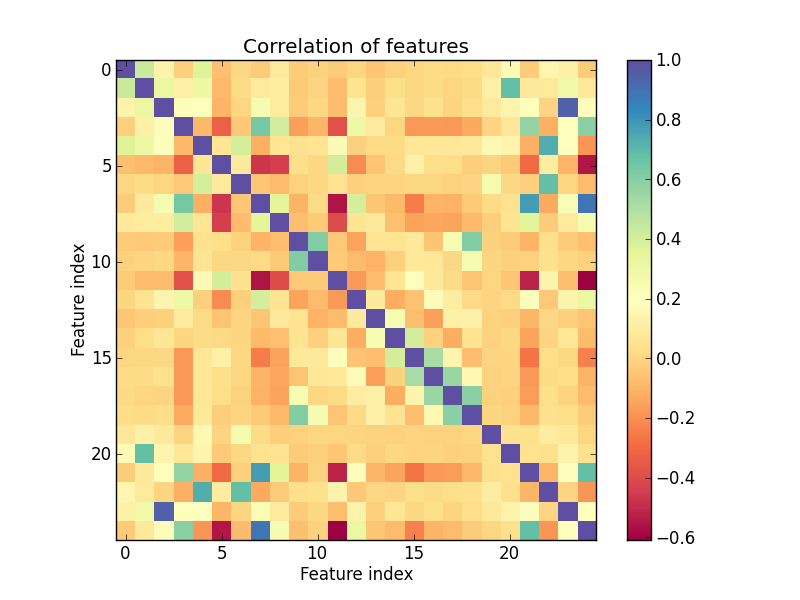
\includegraphics[width=10cm]{correlation_awesome.png}
    \end{center}

    The color of each box (x,y) shows the correlation between features (x,y).
    These are keyed according to the table below.

    \begin{center}
        \begin{tabular}{ |l|l| }
            \hline
            Table Heading                                 & Label Number \\ \hline
            1800 to 2700Hz Band energy                    & 0 \\ \hline
            3500 to 4300Hz Band energy                    & 1 \\ \hline
            5400 to 6800HZ Band Energy                    & 2 \\ \hline
            Dominant Frequency in the 300 to 5000 Hz band & 3 \\ \hline
            Energy of the window                          & 4 \\ \hline
            Kurtosis of the fft                           & 5 \\ \hline
            0 to 100Hz Band Energy                        & 6 \\ \hline
            LPC Component 0                               & 7 \\ \hline
            LPC Component 1                               & 8 \\ \hline
            LPC Component 10                              & 9 \\ \hline
            LPC Component 11                              & 10 \\ \hline
            LPC Component 2                               & 11 \\ \hline
            LPC Component 3                               & 12 \\ \hline
            LPC Component 4                               & 13 \\ \hline
            LPC Component 5                               & 14 \\ \hline
            LPC Component 6                               & 15 \\ \hline
            LPC Component 7                               & 16 \\ \hline
            LPC Component 8                               & 17 \\ \hline
            LPC Component 9                               & 18 \\ \hline
            LPC Residual                                  & 19 \\ \hline
            Peak at 21st PSD component                    & 20 \\ \hline
            PSD dominant component after third component  & 21 \\ \hline
            Sum of PSD components 0 through 3             & 22 \\ \hline
            Sum of PSD components 30 through 36           & 23 \\ \hline
            Zero Crossing rate                            & 24 \\ \hline
        \end{tabular}
    \end{center}

    \caption{Diagram showing correlation between features}
    \label{fig:correlation-awesome}
\end{figure}


From figure \ref{fig:correlation-awesome} we can see that there is a very low
level of correlation between most of the features: the average correlation is
0.04 and the standard deviation is 0.21.

However, some of these variables are highly correlated. This suggests that
perhaps we could remove these features or perform a principal component
analysis to further reduce the dimensionality of the data. Specifically:

\begin{itemize}

    \item 15 and 16 have a correlation of just over 0.5. These features
        represent the $6^{th}$ and $7^{th}$ components of the LPC analysis.
        This result is not entirely unexpected as the LPC attempts to best fit
        the signal, in some signals (such as flat noise) there is very little
        variation needed to predict the next item from the previous 12.

    \item 7 and 11 have a correlation of just over -0.5. These features
        represent the $0^{th}$ and $2^{nd}$ components of the LPC. Again this
        is somewhat expected because some signals will have little variation.

    \item 9 and 10, 18 and 9, and 16 and 11 which are also LPC components
        have a high correlation.

    \item 22 and 4 have a high level of correlation. This represents the sum of
        the first 4 (0-3) PSD components and the energy of the overall 16ms
        window. This can be somewhat explained by the fact that the dominant
        frequency components in the power spectrum lie in these components and
        as such will make up most of the energy of the frame. Whilst
        intuitively this result makes sense, it is worth noting that the sum of
        the 0-3 PSD band gives much more classification importance (see: figure
        \ref{table:importances}) than the energy of the frame. As such it is
        worth keeping both of these features: it is trivial to compute the
        energy (sum of squares) of the frame of audio.

    \item 5 and 24 have a correlation of -0.55. This is a relatively strong
        negative correlation. The kurtosis of the FFT and the zero crossing
        rate are somewhat inherently linked. This is because the whole spectrum
        of the signal will determine the zero crossing rate and the kurtosis
        is a summary statistic of the FFT.

    \item 7 and 21 have a correlation of 0.7800. The 0th LPC coefficient and the
        dominant component of the PSD after the third component are possibly
        linked in that the LPC coefficient will change with frequency
        information and the dominant frequency is obviously directly extracting
        frequency information.

    \item 7 and 24 have a correlation of 0.8900. The 0th LPC coefficient and the
        zero crossing rate are inherently linked: the zero crossing rate
        describes a characteristic that the LPC is trying to accurately
        predict, that is the rate of sign change in the signal.

\end{itemize}

Here we have seen that only 9 pairs of features have correlations of above 0.5.
This is a very encouraging finding as it indicates that the vast majority of
our features present different ``views'' on the data. As such we have a
representation of voice/keyboard noise/background noise that is very amenable
to classification. Independence between features is very important for us: if
two features are highly correlated they do not provide much useful information
for classification. By comparison if the two features are highly uncorrelated
they provide much more information for classification.

\subsection{Analysis of the features with respect to accuracy}

Once we had built our feature representation and tested the features with our
classifier, we decided that the next step in our implementation was to
determine the predictive power of our features. In order to do this we trained
decision trees on each feature individually. The objectives of this exercise were:

\begin{itemize}

    \item To determine how accurately the feature importances reported from the random
        forest classifier represent the predictive power of the individual features.

    \item To show how much stronger the predictive power of the
        combination of all the features is than any individual feature.


    \item To demonstrate that the combination of features performs
        significantly better than just passing the entire frame through as the training
        example.

\end{itemize}

The reports of accuracy here are given by taking the results of a 10 fold, 66\%
training, 33\% test cross validation. Accuracy was determined using the MAE
metric and the standard deviation in this metric also reported.

\begin{figure}
    \begin{center}
        \begin{tabular}{|l|l|l|}
            \hline
            Feature Name                                  & $1-\text{MAE}(\text{Feature})$ & $\text{STDEV}(1-\text{MAE}(\text{Feature}))$ \\ \hline
            1800 to 2700Hz Band energy                    & 0.6113                         & 0.0019 \\ \hline
            3500 to 4300Hz Band energy                    & 0.5762                         & 0.0044 \\ \hline
            5400 to 6800HZ Band Energy                    & 0.5427                         & 0.0029 \\ \hline
            Dominant Frequency in the 300 to 5000 Hz band & 0.6040                         & 0.0031 \\ \hline
            Energy of the window                          & 0.6252                         & 0.0018 \\ \hline
            Kurtosis of the fft                           & 0.5305                         & 0.0063 \\ \hline
            0 to 100Hz Band Energy                        & 0.7063                         & 0.0024 \\ \hline
            LPC Component 0                               & 0.5788                         & 0.0030 \\ \hline
            LPC Component 1                               & 0.5393                         & 0.0043 \\ \hline
            LPC Component 10                              & 0.5123                         & 0.0020 \\ \hline
            LPC Component 11                              & 0.5077                         & 0.0044 \\ \hline
            LPC Component 2                               & 0.5550                         & 0.0029 \\ \hline
            LPC Component 3                               & 0.5186                         & 0.0040 \\ \hline
            LPC Component 4                               & 0.5207                         & 0.0027 \\ \hline
            LPC Component 5                               & 0.5183                         & 0.0030 \\ \hline
            LPC Component 6                               & 0.5150                         & 0.0013 \\ \hline
            LPC Component 7                               & 0.5126                         & 0.0049 \\ \hline
            LPC Component 8                               & 0.5146                         & 0.0049 \\ \hline
            LPC Component 9                               & 0.5074                         & 0.0020 \\ \hline
            LPC Residual                                  & 0.6095                         & 0.0032 \\ \hline
            Peak at 21st PSD component                    & 0.5612                         & 0.0041 \\ \hline
            PSD dominant component after third component  & 0.6017                         & 0.0021 \\ \hline
            Sum of PSD components 0 through 3             & 0.6754                         & 0.0012 \\ \hline
            Sum of PSD components 30 through 36           & 0.5490                         & 0.0016 \\ \hline
            Zero Crossing rate                            & 0.7057                         & 0.0015 \\ \hline
        \end{tabular}
    \end{center}
    \caption{Table showing the relative accuracies of individual features}
    \label{fig:feature-accuracies}
\end{figure}

As we can see (in figure \ref{fig:feature-accuracies}) the 0-100Hz band energy
feature is by far the best predictor within the individual feature set. This
corresponds strongly with the feature importances computed by the classifier.
An interesting upset is that feature 25 also gives a relatively high prediction
rate on its own. The reason for this upset is that the zero crossing rate was
one of the features given the lowest importance by the random forest
classifier. This is particularly interesting, according to the correlation
matrix of features: 6 and 24 are relatively uncorrelated (-0.077). If they
both have strong predictive power, we would expect them to combine together to
give a very good classification accuracy.

It is worth noting that our second best predictor from the importances in
figure \ref{table:importances}, the sum of the first 4 (0-3 inclusive) PSD
components, comes a very close third in this table: with 68.5\% accuracy as
a predictor on its own. The reason that our classification rate is so much
higher than any individual feature combined is: whilst each of the individual
features may not have much better prediction accuracy than the baseline, they
are all somewhat uncorrelated. This means that they present different views on
the data, allowing the random forest classifier to extract nearly all of the
variance from the data set, providing a much more accurate classification.

This section has demonstrated that the features that we have built for our
implementation accurately help us solve the classification problem that we
have: accurately discriminating background noise and typing from human speech.
Based on the results reported here we are confident that this implementation is
very much a working prototype of this system. We believe that some future work
remains in ensuring that this system is robust to new speakers by building a
much larger training set with a much more representative sample of speakers.

\section{The effect of the number of bits for sample}

In the technical background chapter we explained how each sample of audio is
represented by a number of bits, more bits giving much higher fidelity audio
sample. We started with 16 bit audio samples, and in this experiment we
investigate the effect of changing to 8 bits per sample instead. There are a
number of compelling reasons to make this change:

\begin{enumerate}

    \item If the bits per sample can be reduced, the overall data rate going
        through the system will be reduced. This may give performance benefits
        such as being able to apply the feature transformations more quickly
        and fitting more data in the cache lines. Particularly as VAD systems
        are used in embedded/mobile computing contexts, being able to work with
        smaller data sets is important.

    \item Additionally it means that the data set that we use can be more
        aggressively compressed for serving on the internet: we have built a
        unique corpus that includes audio like laughter and keyboard noise.
        These samples were not found in the existing corpora, as such having
        a data set that is more amenable to distribution is a benefit.

\end{enumerate}

We obviously expect to see a reduced classification accuracy from deleting
the lower 8 bits of audio information. It is worth noting that unlike music,
voice tends to have a fairly uniform amplitude. As such the minor variations
may not have that much of an effect.

To perform this experiment we modified the part of the program that reads the
audio from the files. Instead of just passing out the entire audio sample we
masked out the lower 8 bits of the 16 bit sample. This is equivalent to
removing these bits in terms of the effect on the accuracy of the
classification system. In order to perform testing we trained our classifier
system on 50\% of the data in the training set and tested against the other
50\%. The ROC curves of the results from this experiment are shown in
figure \ref{fig:roc-bitcrush}.

\begin{figure}
    \center {
    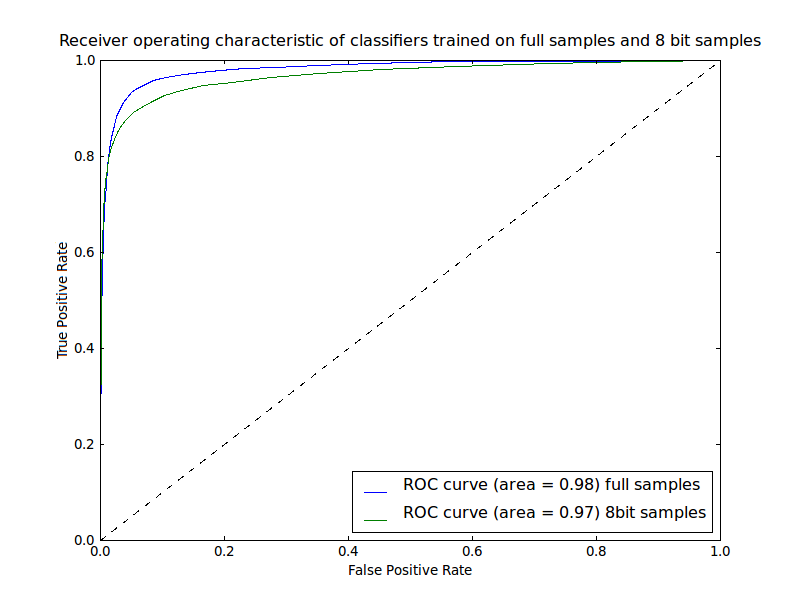
\includegraphics[height=10cm]{roc_8bit.png}
}
    \caption{ROC curves of the two classifiers}
    \label{fig:roc-bitcrush}
\end{figure}

This curve clearly shows that the accuracy of the two classifiers is nearly the
same. Specifically 98\% area under the ROC curve for the full bit samples
versus 97\% area under the ROC curve for 8 bit samples. This finding is useful,
it means that the classifier can be trained on lower bit rate datasets. This
will reduce the overall size of the classification model that has to be loaded
into memory: the full classifier takes 65 megabytes of memory, the reduced one
takes only 40.  This means that, for example, this system could be released on
both PC and embedded contexts. The slightly higher accuracy version could be
released on PC and the lower accuracy version released on the embedded/mobile
devices. One of the main aims of this project is to release our corpus after we
have completed.  It is important to note that reducing the size of the archive
that we release will directly increase the number of people that it is
available to. By halving we think reducing the bitrate is a good way to improve
our ability to release the system and improve processing performance, in exchange
for a small amount of classification accuracy.

\section{The effect of changing audio frame rate}

Changing the frame rate will naturally be expected to alter classifier accuracy
and performance. For example: reducing the frame rate will naturally reduce the
resolution of the Fourier transform. Furthermore lowering the frame rate will
reduce the amount of data that forms the basis of other features which we
compute such as energy of the frame. This may also lead to a reduced
classification accuracy. There is some reason to believe that this may not have
as much impact as changing the bit rate of the classifier, this is due to the
fact that human voice rarely goes above 4kHz, with a Nyquist limit of 8kHz. Our
audio samples being recorded at 48kHz means that we may have vastly much more
information than we need. In order to test this we initially started by taking
half (24kHz) and quarter (12kHz) frame rates, to determine whether or not this
would have a significant affect on classification accuracy. The results are
shown in figure \ref{fig:roc-frameratecrush}.

\begin{figure}
    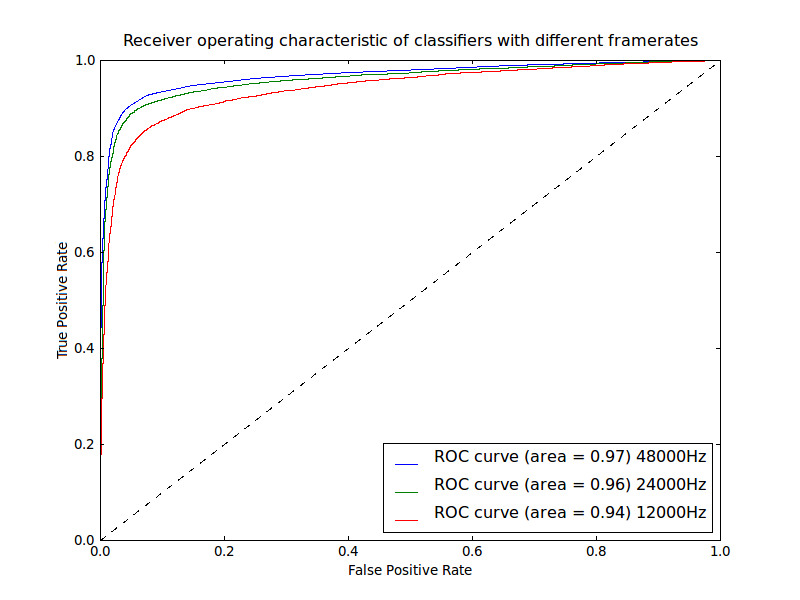
\includegraphics[width=15cm]{roc_framerates.png}
    \caption{ROC curves for various reduced framerates}
    \label{fig:roc-frameratecrush}
\end{figure}

As we can see, the results here are fairly significant. This result is somewhat
counterintuitive. We believe that the explanation for this is that the keyboard
noise contains much higher frequency information than voice. As such cutting
off much of the higher frequency information will degrade our ability to
separate the keyboard and voice classes. This could also be due to the fact
that the features were constructed on 48000Hz audio and that they may need to
be adapted for a lower frame rate.

\section {Robustness to unseen data}

\subsection{Unseen data from seen speakers}

The next question that is important to answer is as to whether the classifier
that we have built is robust to unseen data from seen speakers. If this is the
case one could imagine an automated training scenario whereby the system trains
itself. We would do this by having the user pushing a key to indicate when they
are speaking, transmitting speech when the key is held. This way the system can
build samples in the voice class from the user interaction. After the end of
the training period, however, the system must continue to be robust against
unseen speech from the same user.

For this experiment we used approximately 10 seconds of audio from our sample
data set, with a speaker that the system had already been trained against. This
data was otherwise unseen, it contained some frames where the speaker was
typing and speaking at the same time. Within this sample 222 frames were not
total silence. The sample contained a short, low volume, utterance before the
start of speech. This utterance was picked up by the system and largely
transmitted. The main body of the talking was transmitted and only pauses were
classified as noise. The tail of the speech was also largely transmitted, with
background noise being detected accurately. The classification diagram can be
seen in figure \ref{fig:ultimation}.

\begin{figure}
    \begin{center}
        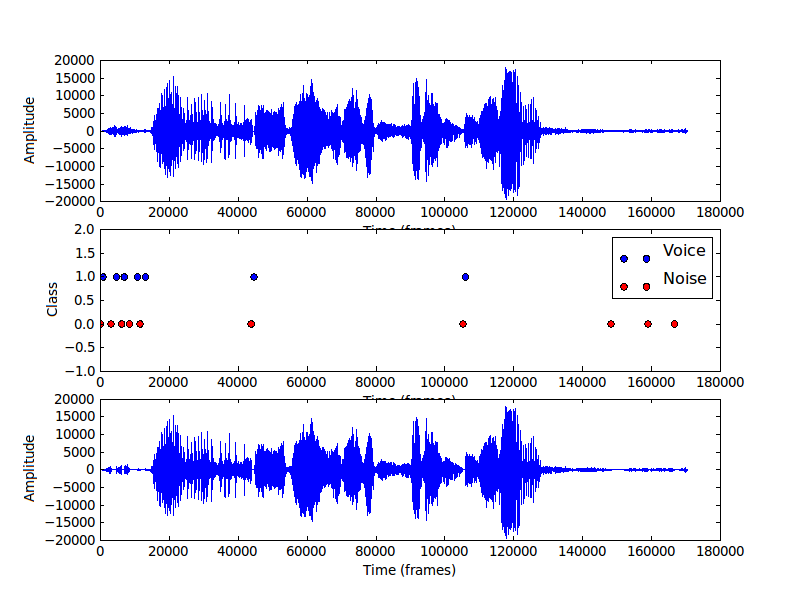
\includegraphics[width=10cm]{ultimation.png}
    \end{center}


    This classification diagram shows the original audio waveform, the class
    predictions that the classifier made (when they changed) and the
    post-processed waveform. Specifically here we can see the classification 0
    frames is noise, the class then bounces back and forth between noise and
    voice during the low amplitude utterence, at $\approx42000$ frames we can
    see the class changes from noise to voice and so on. The post-processed
    waveform has any frames marked as noise by the classifier set to amplitude
    zero. The first two spikes that can be seen are typing impulses, the second
    and final spikes are voice data. As can be seen the noise impulses get
    largely silenced, but the classification during the voice is also very
    noisy.

    This entire sample is considered to be voice data.

    \caption{Classification diagram for unseen data from a seen speaker}
    \label{fig:ultimation}
\end{figure}

This shows us that, firstly, we have built a system that is relatively robust
to speakers that have been seen. Despite the fact that we haven't seen the
specific speech data before. This is encouraging because it indicates that this
system will work where the speaker has been seen before. More importantly, this
indicates that the classifier has a very high level of sensitivity as it
accurately classified the two pauses within the overall speech.

A possible problem that is brought up by this is that very quiet utterances
flick back and forth between the background noise and speech class. This could
be annoying if it repeatedly happens and brings to bear the idea of a smoothing
system/long term classifier. The long term classifier would use more
information from the long term context of speech. This is in contrast to our
system which only uses the short term context of a single 16ms window.

\subsection{Unseen speakers}

It is important to test our classifier with unseen data, these data are a good
way to test possible future performance when the system is used in a production
environment. The classifier system was only trained with 9 speakers. As such
there is a possibility that it will not work well with when presented with
unseen speakers. To test this we recorded a sequence of audio. It contained
both speech and keyboard impulses. The speaker was an unseen, male, speaker.
The sequence was approximately approximately 16.5 seconds in length. This gave
us 1037 windows to classify against the unseen speaker. The classifier was
trained against the entire labelled training set that we created. We then
performed classification on each of the frames in the unseen sequence. The
confusion matrix for this experiment can be seen in figure
\ref{table:confusion_unseen}. We discard totally silent windows, this means
that of the 1037 we had, only 822 windows were seen by the classifier. From a
visual inspection of the data in figure \ref{fig:waveform_unseen} we can see
that noise regions were correctly classified, with only a few frames noise
frames being transmitted. Most voice regions were classified noisily. In order
to improve this system to generalize to unseen speakers we would require a much
much larger sample of audio to draw from. However, hand labelling may
significantly slow the process.


\begin{figure}
    \begin{center}
        \begin{tabular}{| l | l | l |}
            \hline
                         & Predicted Voice & Predicted Noise \\ \hline
            Actual Voice & 43              & 123 \\
            Actual Noise & 40              & 616 \\ \hline
        \end{tabular}
    \end{center}
    \vspace{\baselineskip}

    The confusion matrix indicates that the classification is very good at
    classifying background noise, but not so good at classifying speech. This
    result is expected: it indicates that there is much more variation in the
    voice of an unseen speaker than the background noise of an unseen
    configuration. This is due to the fact that additive background noise is
    largely the same in any environment. Background noise is picked up, in
    different ways, due to the different sensitivities of microphones.

    \caption{Confusion matrix for unknown speaker}
    \label{table:confusion_unseen}
\end{figure}

\begin{figure}
    \begin{center}

        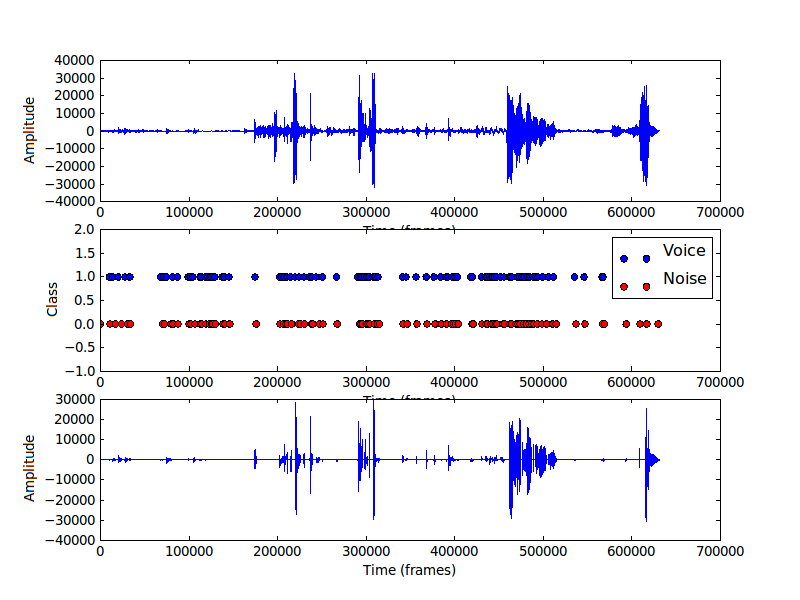
\includegraphics[width=10cm]{peter.png}
    \end{center}

    This classification diagram works in a similar way to the previous one. The
    first two spikes on this diagram are keyboard noise, the final spikes are
    both voice data. As we can see the classification is very spotty.

    \caption{Classification diagram for unseen speaker}
    \label{fig:waveform_unseen}

\end{figure}

Critically we see that the system that we have trained is not immediately
robust to new speakers. This is important because it implies that our
implementation, whilst giving good accuracy on speakers that it has seen, is
not yet ready for unseen speakers. Our expectation is that if we provide more
data to train against the system would be ready to handle unseen speakers.

\section{Performance of different classification algorithms}

The choice to use the Random Forest classification algorithm was very much a
decision made based on the author's experience. In this section we aim to see
whether any of the other classification techniques mentioned in the technical
background section prove to give a better classification rate on the data set.
Whilst the features were very much generated with a random forest in mind, we
have shown that the features themselves give relatively independent views on
the data set.

With this in mind, we decided to use all of the ensemble methods discussed
earlier, a simple decision tree algorithm and the k nearest neighbor method.
These represent a broad stroke of classification algorithms used today and will
hopefully reveal as to whether or not our decision to use the Random Forest
classifier was a correct one. For all classifiers we have reported the ROC
curves in figure \ref{fig:multiclass-roc}, the confusion matrices in
figure \ref{fig:multiclass-confusion} and the training and test times in
figure \ref{fig:multiclass-speed}. This experiment was performed by training the
classifiers on half of the data that we have available and using the other half
as unseen testing examples.

\begin{figure}
    \begin{center}
        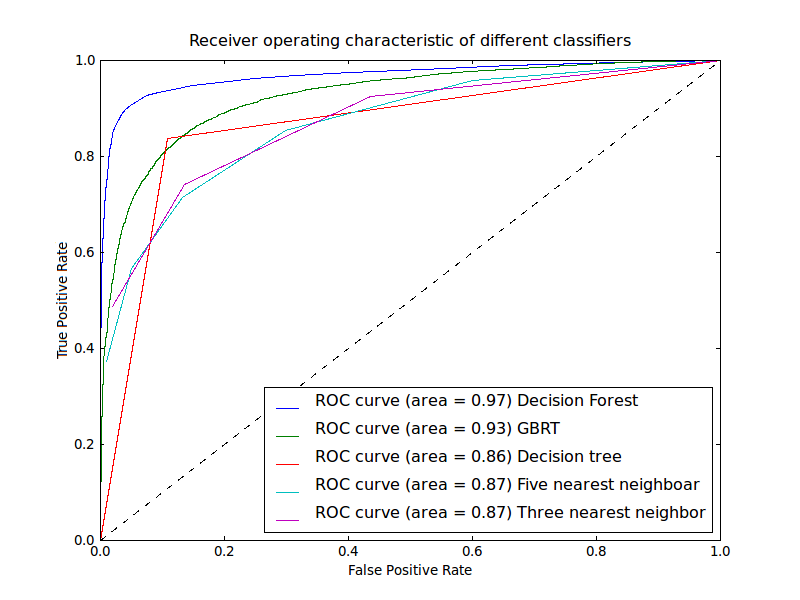
\includegraphics[width=10cm]{roc_different.png}
    \end{center}
    \caption{ROC curves of different classifiers}
    \label{fig:multiclass-roc}
\end{figure}

\begin{figure}

    \center{
    \begin{tabular}{|l||l|l|}
        \hline
        Random Forest      & Actually Positive & Actually Negative \\ \hline
        Predicted Positive & 9712              & 288               \\ \hline
        Predicted Negative & 1244              & 8756              \\ \hline
    \end{tabular}

    \vspace{0.7500cm}

    \begin{tabular}{|l||l|l|}
        \hline
        GBRT               & Actually Positive & Actually Negative \\ \hline
        Predicted Positive & 9209              & 791               \\ \hline
        Predicted Negative & 2291              & 7709              \\ \hline
    \end{tabular}

    \vspace{0.7500cm}

    \begin{tabular}{|l||l|l|}
        \hline
        Decision tree      & Actually Positive & Actually Negative \\ \hline
        Predicted Positive & 8912              & 1088               \\ \hline
        Predicted Negative & 1633              & 8367              \\ \hline
    \end{tabular}

    \vspace{0.7500cm}

    \begin{tabular}{|l||l|l|}
        \hline
        Five Nearest Neighbor & Actually Positive & Actually Negative \\ \hline
        Predicted Positive    & 8684              & 1316               \\ \hline
        Predicted Negative    & 2861              & 7139              \\ \hline
    \end{tabular}

    \vspace{0.7500cm}

    \begin{tabular}{|l||l|l|}
        \hline
        Three Nearest Neighbor & Actually Positive & Actually Negative \\ \hline
        Predicted Positive     & 8642              & 1358               \\ \hline
        Predicted Negative     & 2590              & 7410              \\ \hline
    \end{tabular}

    \vspace{0.7500cm}

}
    \caption{Confusion matrices for different classifiers}
    \label{fig:multiclass-confusion}

\end{figure}

\begin{figure}
    \center{
    \begin{tabular}{|l|l|l}
        \hline
        Classifier             & Training Time (seconds) & Testing time (seconds) \\ \hline
        Random Forest          & 7.83                    & 0.47 \\
        GBRT                   & 1.69                    & 0.26 \\
        Decision Tree          & 0.35                    & 0.12 \\
        Three Nearest Neighbor & 0.16                    & 18.12 \\
        Five Nearest Neighbor  & 0.16                    & 18.13 \\
    \end{tabular}
}

    \caption{Training and testing times for various classifiers}

    \label{fig:multiclass-speed}
\end{figure}

The reason this experiment is important is that if we can achieve a better
classification accuracy, or classification performance in time/memory with any
of these systems, then using that classifier would be preferable. The first
thing we note is that the Random Forest gives the best classification rate by
some measure and is followed by the Gradient Boosted Regression Trees
algorithm. This does not contravene expectations as these methods both use a
large ensemble of classifiers. Specifically for both ensemble classifiers we
trained using 100 trees.

We note that the Extremely Random Forest is not shown here. This is because it
had  extremely similar accuracy and performance characteristics to the Random
Forest. Adaboost is not shown as we had trouble getting it to successfully
classify on our dataset. We believe this is because it is currently not in a
stable release of the SKLearn library.

What is more interesting is perhaps that the decision tree classifier achieves
a higher raw classification accuracy than all the algorithms apart from the
decision forest, but the decision tree algorithm has a lower area under the ROC
curve. This is because the classifier implementation that we used for the
Decision Tree does not provide output probabilities but rather a ${0,1}$
discrete classification. This means that its potentially more accurate
classification suffers under the ROC curve metric. This is because it must be
linearly interpolated to the (0,0) and (1,1) points from its actual
classification output. By comparison we can see that the ROC AUC metric favours
the lower accuracy five nearest and three nearest neighbor classifiers because
they return continuous predictions instead of discrete output.

If we look at the confusion matrices of these 4 classifiers we can see
that that the decision tree actually gives a much better overall classification
rate than the five nearest neighbor. These are all important factors to
consider when deciding which classifier to use. For example the GBRT
implementation classifies about twice as fast as the random forest
implementation (0.4700 seconds versus 0.2600 seconds) and has a somewhat lower
accuracy.

From this we can, however, immediately discard the 3 nearest and 5 nearest
neighbor classifiers, they take both the longest to classify (18 seconds
respectively to classify 320 seconds of audio) and give the lowest
classification accuracy. Although 18 seconds for 320 seconds of audio may seem
like reasonable performance, we envisage this system sitting in amongst many
other components of a VOIP stack and introducing any latency may have an impact
on user experience. Certainly the more latent any particular component is, the
more optimised the other components have to be.

All three tree implementations run in under a second with the decision tree
algorithm running in 0.12 seconds, the GBRT running in 0.26 and the Random
forest running in 0.47 seconds. All of these implementations have a very high
classification accuracy and classification speed, and any of them could be used
for a real time system. The result of the Random Forest running more slowly
than the GBRT is somewhat counterintuitive because our Random Forest runs in
parallel. It performed more slowly in both multiprocessing and serial
modes, so we assume that something about the reduction of the classifier voting
takes longer than pushing an example through the decision chain in the GBRT.
The authors' recommendation would be to use the decision forest implementation
because it is both the most accurate overall, has the best area under the ROC
curve and it has a very high performance.

\section{Varying the number of estimators in the ensemble}

The random forest classifier takes two parameters. These parameters are the
number of trees to train and the maximum depth to which to train the trees. In this
section we investigate the effect on classification accuracy of training more
trees. We explicitly do not investigate processing performance of the
classifier as the relationship between number of estimators and performance is
essentially linear.

In order to perform this experiment we used the same 50\% training, 50\% test
split that was used before. The system was trained with 500 trees, as well as
100 through 10 trees in steps of 5. The reason for training 500 trees is to see
whether having a huge number of extra trees helps. Generally speaking the more
highly trained the classifier is, the more overfit to the training set it may
be. In addition to this there is a disadvantage to training more trees: the
model will take up more memory and disk space, and take longer to process
instances. All other tree counts are used to help us determine if 100
estimators is a reasonable choice of estimator count for our classifier.

The results of this experiment are reported by comparing the ROC AUC to the
number of trees that were trained in the classifier, they are shown in
figure \ref{fig:roc-trees}.

\begin{figure}
    \center{
    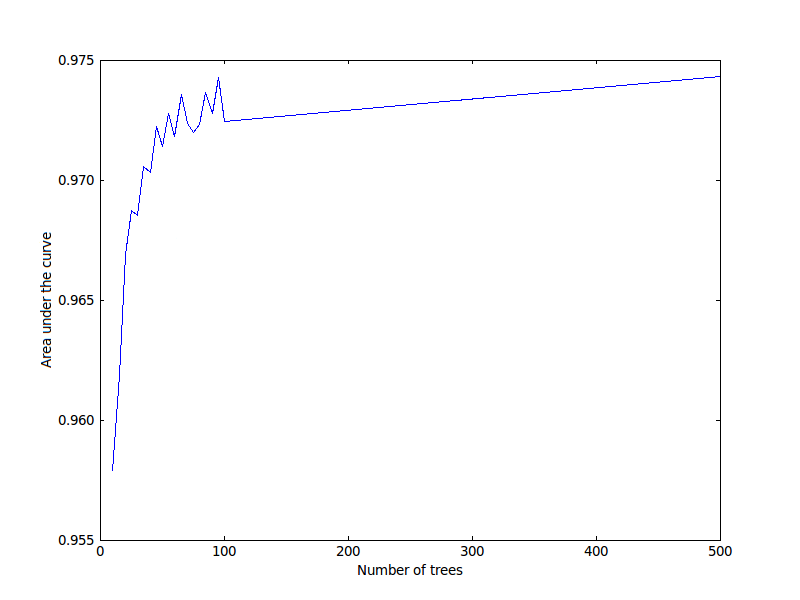
\includegraphics[width=10cm]{roc_differing_trees.png}}
    \caption{ROC area under curve for different trees}
    \label{fig:roc-trees}
\end{figure}

500 trees is slightly more accurate than 95 trees: 0.97431 for 95 versus
0.97426 but at this point we are into diminishing returns. We would not consider
this to be a significant difference in classification accuracy.

An interesting observation we make with this graph is that in general the odd
numbered counts of trees seem to cause peaks in accuracy when compared with
their even numbered counterparts. An example of this is shown in figure
\ref{table:roc_spike}, the table shows the last 4 points in the curve, with
their ROC AUC scores.

\begin{figure}
    \center{
    \begin{tabular}{|l|l|}
        \hline
        Number of trees & ROC AUC \\ \hline
        500             & 0.9743 \\ \hline
        100             & 0.9724 \\ \hline
        95              & 0.9743 \\ \hline
        90              & 0.9728 \\ \hline
        85              & 0.9737 \\ \hline
    \end{tabular}
}
    \caption{ROC AUC metrics for various numbers of trees}
    \label{table:roc_spike}
\end{figure}

This result is somewhat counterintuitive as we would generally expect more
trees to give a better classification result. It is possible that the
``voting'' process of the random forest favours odd numbers, as a way of
breaking ties.  These differences are so small that we decided to employ a
t-test to determine the whether the differences were significant. The test was
performed over the 10 fold cross validation results of two classifiers, one
trained with 100 trees and one trained with 95 trees. In order to do this we
use the standard difference of two means test. The test's results are shown in
figure \ref{fig:t-test}.

\begin{figure}
    \center {
    \begin{tabular}{|l|l|l|}
        \hline
        Number of trees & Mean accuracy in cross validation & StDev accuracy in cross validation \\ \hline
        100             & 0.8900                            & 0.0025                             \\ \hline
        95              & 0.8902                            & 0.0012                             \\ \hline
    \end{tabular}

    $$H_0:\mu_1-\mu_2=0$$
    $$H_1:\mu_1-\mu_2>0$$

    The z score is:

    $$z=\frac{0.8900\times0.8902}{\sqrt{\frac{10\times0.0250+10\times0.0012}{10+10-2}}\times\sqrt{\frac{10+10}{10\times10}}}=-0.0008$$
}

    This is nowhere near high enough for us to conclude statistical significance and so we assume these come from the same distribution.

    \caption{t-test for whether a forest with 95 trees is better than a forest with 100 trees}

    \label{fig:t-test}

\end{figure}

Whilst it is interesting to note the spikeyness, the t-test's results show that
the spikes are not significant. Obviously, more trees lead to a reduction in
processing performance as a tradeoff for classification accuracy.  We think
that using 100 trees is a sensible default. It was also the number of trees the
system implemented with.  We would definitely use this estimator count going
forward. The reason for this is we designed our features with this estimator
count. Additionally no other estimator count seems to give a better
classification accuracy.

\section{Varying the maximum depth of the classifier}

A commonly used technique for reducing overfitting of a decision tree
classifier is to prune the trees to a specified
depth\cite{Bramer:2002:PCT:646288.686755}. This works because decision trees
train until all the leaf nodes in the tree are of uniform class. This leads to
a very high level of bias to the specific data set that the tree has been
trained on. The random forest is somewhat robust to this problem because it
trains many trees on different samples of the original data
set.\footnote{Random forests train each tree by sampling the original data set
with replacement} As such it is common to train random forests to the maximum
depth, instead of pruning them.

In this section we will investigate whether pruning our forest helps. For this
experiment we used the 100 tree forest. This size of forest was used during the
execution phase of this project. Depths were chosen between 10 and 1000 (in
steps of 50) and we also trained a completely unpruned forest. The graph of
results shows a comparison of the pruning depth with the ROC AUC metric. The
maximum depth tree is not included in this graph as it is not clear what depth
it was grown to.  The graph is shown in figure \ref{fig:roc-depths}.

\begin{figure}
    \begin{center}
        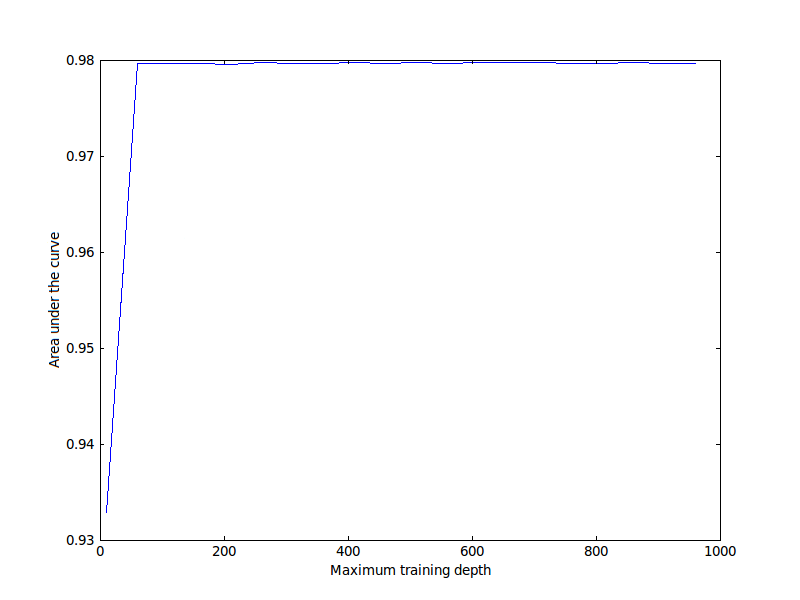
\includegraphics[width=10cm]{roc_differing_depth.png}
    \end{center}

    \caption{ROC AUC metrics for different tree depths}
    \label{fig:roc-depths}
\end{figure}

As we can see from this curve that after a depth of 60 we hit the accuracy
limit of around 0.98. It is worth noting that there appears to be an accuracy
limit around 98\%, regardless of how deep we allow the classifier to train.
From this we can conclude that classifier depth does not have a significant
effect on classification accuracy. As such we would recommend either using a
pruning depth of around 200 or not pruning. The justification for not pruning
is that our features were trained with unpruned trees. The justification for
pruning to a maximum depth of 200 is that the classifier will be of reduced
size, which will enable faster classification times.

\section{Comparison with existing VAD algorithms}

In this section we compare our system to other VAD algorithms, for the most
part we did not directly implement other VAD algorithms. Instead in this
section we perform a comparative analysis on any accuracy values reported in
the papers discussing other algorithms. We compare our system against a system
that implements energy and zero crossing rate. For this comparison we used our
dataset for training and testing. Whilst we have noted that the zero crossing
rate did have a very high level of individual predictive power (approximately
70\%), it was given a relatively low importance by the random forest
classifier.  This indicates that it may not be a very good separator for our
dataset.

In \cite{shin} they report their highest accuracy as a combination of all their
features. The features are used in a combination with a system that passes both
the next and previous frame into their classifier. Our system explicitly does
not take any other frames than the current one. The reason for this design
decision was: we felt that introducing an additional 16ms of latency into the
audio processing would needlessly reduce the performance of the system. In
other words we felt that the possible classification rate gain that we would
achieve would not outweigh the cost of delaying the processing. VAD systems
live or die based on how fast they can process data. In \cite{shin} the
specific accuracy they report with the 0dB noise level \footnote{A noise level
of 0dB is equivalent to the spoken audio being as loud as the background noise}
is 87.7300\%. Our highest classification accuracy in cross validation was 91\%,
we also have noise attenuated to roughly the same 0dB level.  We feel that the
reason that our system is more accurate than the system in \cite{shin} is that
we have used a very advanced machine learning algorithm, the random forest,
instead of the decision tree. Additionally we have more features: their system
uses only 6 features instead of 25. It is worth noting that this may mean that
the performance of our system is worse, we have, however, experimentally
determined that our system runs in faster than real time. We are not concerned
with performance issues in our system.

In \cite{moattar} they built a threshold based VAD system, interestingly it was
not tested against English speech but Farsi speech. This means that a direct
comparison of accuracies is not possible as we have not trained our system
against a Farsi corpus. They report approximately\footnote{\cite{moattar} did
not report 0dB attenuated noise accuracies and so figures here are reported by
linearly interpolating between the 5dB and -5dB values.} 86\% accuracy for
their system with white noise at 0dB. This system is much more simple than the
\cite{shin} system and so the accuracy is slightly degraded. It is worth noting
that this system uses much more long term information than the \cite{shin}
system. Specifically it uses approximately 30 frames to make a decision. This
system does not, however, introduce 30 frames of latency as it is threshold
based.

The features of energy and zero crossing rate were the two most used features
from the literature. We decided to compare the predictive power of these two
features with our classifier. In order to do this we trained both the full
classifier and the classifier with these two features against half of the data
that we had labelled.  We then tested the classifiers against the other half of
the data. The results are shown as ROC curves in figure \ref{fig:reduced-features}. As
we can see these combined features give a 91\% area under the ROC curve. Whilst
this predictive power is good, our system performs significantly better. This
indicates that our system has improved on the core predictive features. It is
worth noting that energy has been found to degrade in noisy environments, these
environments being the ones that we are specifically targeting.


\begin{figure}
    \center{
        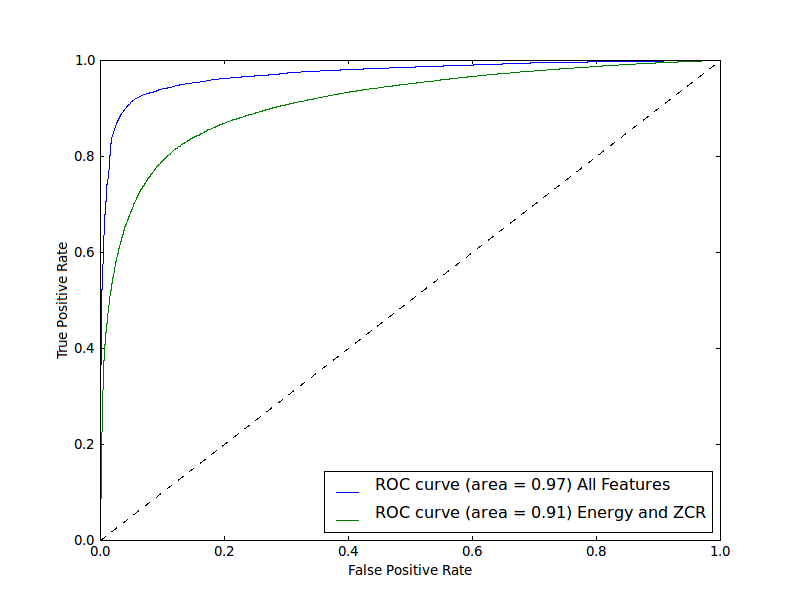
\includegraphics[width=10cm]{roc_reduced_features.png}
    }

    \caption{ROC curves of two classifiers, one trained on energy and ZCR and
    one trained on all features}
    \label{fig:reduced-features}
\end{figure}


Our system compares favourably to these systems. The reason we have done this
investigation is to attempt to gain an understanding of the effects of noise on
VAD systems in general. This result means that our system has somewhat improved
on the state of the art. We have solved a new problem and improved on the
accuracy of most systems from the research. There is one caveat here: our
training set is relatively small, the classification accuracy may get worse as
more data is added. The reason for this is that bigger data sets are generally
more statistically sparse. As such our classifier may be taking advantage of
the small data set size to come to a very accurate classification.

%\noindent This chapter is intended to evaluate what you did.  The content is
%highly topic-specific, but for many projects will have flavours of the
%following:
%
%\begin{enumerate} \item functional testing, inc. analysis of failure cases,
%\item performance results, and analysis of said results that draw some form of
%conclusion, and \item evaluation of options and decisions within the project,
%and/or a comparison with alternatives.  \end{enumerate}
%
%\noindent This chapter often acts to differentiate project quality: even if
%the work completed is of a high technical quality, critical yet objective
%evaluation and comparison of the outcomes is crucial.  In essence, the reader
%wants to learn something, so the worst examples amount to simple statements of
%fact (e.g., ``graph X shows the result is Y''); the best examples are
%analytical and exploratory (e.g., ``graph X shows the result is Y, which means
%Z; this contradicts [1], which may be because I use a different assumption'').
%As such, both positive {\em and} negative outcomes are valid {\em if}
%presented in a suitable manner.

% -----------------------------------------------------------------------------

\chapter{Conclusion}
\label{chap:conclusion}

\section{Review of contributions}

In this project we set out to build a new data set for Voice Activity
Detection.  The dataset to enabled us to build a voice activity detector that
could accurately distinguish human speech from background noise.  Additionally
we wanted to distinguish keyboard noise in personal computing environments. We
also set out to actually build the detector itself.


One of the aims of the project was to explore a new space in voice activity
detection.  Specifically we wanted to be able to distinguish sudden impulses,
as well as background noise of a roughly stationary amplitude. This breaks with
the objectives of most detectors, which only attempt to differentiate
background noise from speech. We wanted to build a system that could robustly
distinguish speech from noise associated with common peripherals, such as mice
and keyboards.

The dataset that we built is in a relatively portable form, 48kHz 16 bit WAV
files, with a separate sqlite3 database holding the information about audio
class and time. The size of the labelled dataset is relatively small, around 1
hour, with a total of 24 hours of audio in the dataset. We believe that a
further contribution that could be made would be for someone to label the rest
of the data set. The labelled data was very much not the primary goal of this
project, this is why a relatively small amount of the data set is actually
labelled. We also investigated the possibility of reducing the size of this
dataset with a view to publishing it, specifically in a format that might
benefit other researchers. Based on our investigation: halving the bits per
sample of the audio from 16 bit to 8 bit should have a very small effect on
future classification. Our feeling is that publishing this corpus may further
help VAD research and we are very interested in publishing it.

One of the other main achievements of this project is building a classifier
that capable of accurately distinguishing human speech from the background
noise classes, we have already discussed this at length. Our feeling is that
our choice of classifier (the random forest) has hugely benefited the
classification accuracy of this project. It has enabled us to classify data
with a very high degree of accuracy, specifically some 4\% over the best
classifier found in the background research\cite{shin}. This is a somewhat
expected result from the use of advanced ensemble machine learning techniques.
We have also contributed an evaluation of which classification systems perform
best over this dataset. Particularly we have shown that nearest neighbor
classifiers perform badly on our data set. Nearest neighbor classifiers work in
a very similar way to the threshold based systems that are occasionally used
for VAD systems. As such we feel that more modern approaches to VAD systems
should not use threshold or neighbor based approaches, instead favouring more
modern machine learning techniques such as ensemble methods.

We have also contributed some significant research into features that work well
for VAD, our specific, non-stationary noise problem. Specifically we have shown
that the somewhat untraditional features of the very low frequency band,
0-100Hz frequency domain energy band and components 0-3 of the PSD, provide
very good classification accuracy. We have also shown that the more traditional
features such as window energy degrade in the presence of loud, sudden noises.
Degradation of this feature was particularly noticeable with the presence of
keyboard noise. We feel that the particular combination of 25 features that we
used give a very good cross spectrum classification that makes our classifier
amenable to many voice related problems. This is because a number of our
features are not targeted at our background noise class but rather our voice
class.

\section{Project Status}

The status of our project is that we have implemented nearly all of the
technology needed for our VAD system. We had originally intended to implement a
long time classifier, sometimes referred to as a hangover system. The idea of
these systems is to smooth the transition between transmission and
non-transmission classes. Our system does give a somewhat back and forth
classification when it encounters ambiguous low amplitude voice frames. We
believe that this could be the site of some future research, certainly based on
some experience a median filter may be sufficient to simply remove this spotted
noise.

The remainder of our aims have been totally implemented. We have built a very
simple script to enable us to label voice versus other types of noise, with the
script we can do this both accurately and quickly. This script is what enabled
us to build our corpus to train the classifier against, we have used this to
build our classifier. As outlined above we would like to see this corpus used
by others to build future classifiers, more specifically to extend this corpus
to build a system that is robust to unseen speakers and potentially unseen
languages.

The major aim of this project was to build a classifier that has a high
accuracy when classifying voice frames against the noise and keyboard frames.
We feel that our implementation completely satisfies this aim, specifically the
classifier that we have built runs in better than real time. We also have shown
that the feature transformations that we have created also run in better than
real time.

Another minor aim of this project that we have achieved was to build a set of
features that can be processed more easily than the entire audio window.  It
is, obviously, important that these features present a view of the data that is
amenable to classification.  Obviously during a machine learning project the
classifier and the features are built hand in hand. Given that we have achieved
a high level of classification accuracy we feel that our feature design has
been very successful.

\section{Future work}

Much of the work of this thesis was in designing features that allow the
classification system to extract all of the variance of the data set. The
handcrafted feature design was effectively a dimensionality reduction from 768
to 25. These features retain much of the information present in the raw audio
data. It is possible that instead of doing explicit feature design we could
pass the entire data set into to what is known as a "hash
kernel"\cite{Weinberger}. This is a way of building a dimensionality reduction
from a hash function. It may be possible to build a feature set from a hash
kernel rather than by hand crafting. Future work could possibly involve
building a VAD system that uses hash kernels instead of handcrafted features.
This may be useful because the current features may not solve future problems:
a hash kernel would contain all of the information needed and as such would be
robust to future problems.

In the future we would also like to see this prototypical system taken forward
to be used in a production environment. This project was born out of
frustration with existing VAD systems detecting keyboard impulses as actual
voice. As such the integration of this system with either the Skype or Mumble
systems would be possible. Before this can happen the corpus that we created
would need to be expanded to include many different speakers including more
females and more than one language (English). Based on all of our analysis,
though, we see no reason why this shouldn't be possible.

In conclusion: we feel that this system has been implemented effectively,
solving a practical problem that exists in the landscape of personal computing.
We have created features that are mostly orthogonal to each other providing a
really useful view on the dataset that we have created. We have also created a
classifier that uses these features to provide a very highly accurate
classification. The VAD system that we have built is truly robust to noisy
personal computing environments with the caveats that we have stated earlier in
this paper and we feel that our implementation is a success.


%\vspace{1cm} 
%
%\noindent
%The concluding chapter of a thesis is often underutilised, in part because
%it is often left until close to the deadline and hence does not get enough 
%attention.  Ideally, the chapter will consist of three parts:
%
%\begin{enumerate}
%\item (Re)summarise the main contributions and achievements, in essence
%      summing up the content.
%\item Clearly state the current project status (e.g., ``X is working, Y 
%      is not'') and evaluate what has been achieved with respect to the 
%      initial aims and objectives (e.g., ``I completed aim X outlined 
%      previously, the evidence for this is within Chapter Y'').  There 
%      is no problem including aims which were not completed, but it is 
%      important to evaluate and/or justify why this is the case.
%\item Outline any open problems or future plans.  Rather than treat this
%      only as an exercise in what you {\em could} have done given more 
%      time, try to focus on any unexplored options or interesting outcomes
%      (e.g., ``my experiment for X gave counter-intuitive results, this 
%      could be because Y and would form an interesting area for further 
%      study'').
%\end{enumerate}

% =============================================================================

% Finally, after the main matter, the back matter is specified.  This is
% typically populated with just the bibliography.  LaTeX deals with these
% in one of two ways, namely
%
% - inline, which roughly means the author specifies entries using the 
%   \bibitem macro and typesets them manually, or
% - using BiBTeX, which means entries are contained in a separate file
%   (which is essentially a databased) then inported; this is the 
%   approach used below, with the databased being thesis.bib.
%
% Either way, the each entry has a key (or identifier) which can be used
% in the main matter to cite it, e.g., \cite{X}, \cite[Chapter 2}{Y}.

\backmatter

\bibliography{thesis}

% -----------------------------------------------------------------------------

% The thesis concludes with a set of (optional) appendicies; these are the
% same as chapters in a sense, but once signaled as being appendicies via
% the associated macro, LaTeX manages them appropriatly.

\appendix

% =============================================================================

\end{document}

